\hypertarget{functionals}{%
\chapter{Functionals}\label{functionals}}

\begin{quote}
``To become significantly more reliable, code must become more
transparent. In particular, nested conditions and loops must be viewed
with great suspicion. Complicated control flows confuse programmers.
Messy code often hides bugs.''

--- Bjarne Stroustrup
\end{quote}

A higher-order function is a function that takes a function as an input
or returns a function as output. We've already seen one type of higher
order function: closures, functions returned by another function. The
complement to a closure is a \textbf{functional}, a function that takes
a function as an input and returns a vector as output. Here's a simple
functional: it calls the function provided as input with 1000 random
uniform numbers. \index{functionals}

\begin{Shaded}
\begin{Highlighting}[]
\NormalTok{randomise <-}\StringTok{ }\ControlFlowTok{function}\NormalTok{(f) }\KeywordTok{f}\NormalTok{(}\KeywordTok{runif}\NormalTok{(}\FloatTok{1e3}\NormalTok{))}
\KeywordTok{randomise}\NormalTok{(mean)}
\end{Highlighting}
\end{Shaded}

\begin{verbatim}
## [1] 0.506
\end{verbatim}

\begin{Shaded}
\begin{Highlighting}[]
\KeywordTok{randomise}\NormalTok{(mean)}
\end{Highlighting}
\end{Shaded}

\begin{verbatim}
## [1] 0.501
\end{verbatim}

\begin{Shaded}
\begin{Highlighting}[]
\KeywordTok{randomise}\NormalTok{(sum)}
\end{Highlighting}
\end{Shaded}

\begin{verbatim}
## [1] 489
\end{verbatim}

The chances are that you've already used a functional: the three most
frequently used are \texttt{lapply()}, \texttt{apply()}, and
\texttt{tapply()}. All three take a function as input (among other
things) and return a vector as output.

A common use of functionals is as an alternative to for loops. For loops
have a bad rap in R. They have a reputation for being slow (although
that reputation is only partly true, see
\protect\hyperlink{modification}{modification in place} for more
details). But the real downside of for loops is that they're not very
expressive. A for loop conveys that it's iterating over something, but
doesn't clearly convey a high level goal. Instead of using a for loop,
it's better to use a functional. Each functional is tailored for a
specific task, so when you recognise the functional you know immediately
why it's being used. Functionals play other roles as well as
replacements for for-loops. They are useful for encapsulating common
data manipulation tasks like split-apply-combine, for thinking
``functionally'', and for working with mathematical functions.
\index{for loops}

Functionals reduce bugs in your code by better communicating intent.
Functionals implemented in base R are well tested (i.e., bug-free) and
efficient, because they're used by so many people. Many are written in
C, and use special tricks to enhance performance. That said, using
functionals will not always produce the fastest code. Instead, it helps
you clearly communicate and build tools that solve a wide range of
problems. It's a mistake to focus on speed until you know it'll be a
problem. Once you have clear, correct code you can make it fast using
the techniques you'll learn in \protect\hyperlink{profiling}{improving
the speed of your code}.

\hypertarget{outline}{%
\paragraph{Outline}\label{outline}}

\begin{itemize}
\item
  \protect\hyperlink{lapply}{My first functional: lapply()} introduces
  your first functional: \texttt{lapply()}.
\item
  \protect\hyperlink{functionals-loop}{For loop functionals} shows you
  variants of \texttt{lapply()} that produce different outputs, take
  different inputs, and distribute computation in different ways.
\item
  \protect\hyperlink{functionals-ds}{Data structure functionals}
  discusses functionals that work with more complex data structures like
  matrices and arrays.
\item
  \protect\hyperlink{functionals-fp}{Functional programming} teaches you
  about the powerful \texttt{Reduce()} and \texttt{Filter()} functions
  which are useful for working with lists.
\item
  \protect\hyperlink{functionals-math}{Mathematical functionals}
  discusses functionals that you might be familiar with from
  mathematics, like root finding, integration, and optimisation.
\item
  \protect\hyperlink{functionals-not}{Loops that shouldn't be converted
  to functions} provides some important caveats about when you shouldn't
  attempt to convert a loop into a functional.
\item
  \protect\hyperlink{function-family}{A family of functions} finishes
  off the chapter by showing you how functionals can take a simple
  building block and use it to create a set of powerful and consistent
  tools.
\end{itemize}

\hypertarget{prerequisites}{%
\paragraph{Prerequisites}\label{prerequisites}}

You'll use closures frequently used in conjunction with functionals. If
you need a refresher, review \protect\hyperlink{closures}{closures}.

\hypertarget{lapply}{%
\section{My first functional: lapply()}\label{lapply}}

The simplest functional is \texttt{lapply()}, which you may already be
familiar with. \texttt{lapply()} takes a function, applies it to each
element in a list, and returns the results in the form of a list.
\texttt{lapply()} is the building block for many other functionals, so
it's important to understand how it works. Here's a pictorial
representation: \indexc{lapply()}

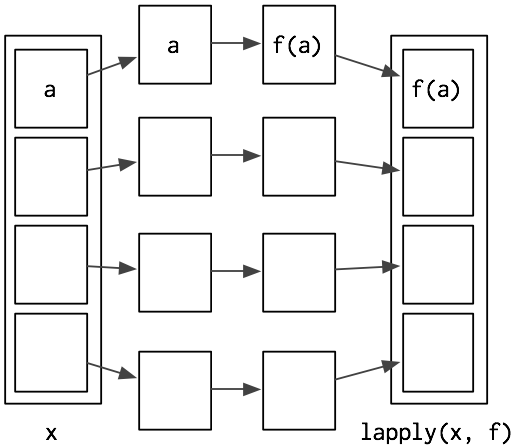
\includegraphics[width=2.4in]{diagrams/lapply.png}

\texttt{lapply()} is written in C for performance, but we can create a
simple R implementation that does the same thing:

\begin{Shaded}
\begin{Highlighting}[]
\NormalTok{lapply2 <-}\StringTok{ }\ControlFlowTok{function}\NormalTok{(x, f, ...) \{}
\NormalTok{  out <-}\StringTok{ }\KeywordTok{vector}\NormalTok{(}\StringTok{"list"}\NormalTok{, }\KeywordTok{length}\NormalTok{(x))}
  \ControlFlowTok{for}\NormalTok{ (i }\ControlFlowTok{in} \KeywordTok{seq_along}\NormalTok{(x)) \{}
\NormalTok{    out[[i]] <-}\StringTok{ }\KeywordTok{f}\NormalTok{(x[[i]], ...)}
\NormalTok{  \}}
\NormalTok{  out}
\NormalTok{\}}
\end{Highlighting}
\end{Shaded}

From this code, you can see that \texttt{lapply()} is a wrapper for a
common for loop pattern: create a container for output, apply
\texttt{f()} to each component of a list, and fill the container with
the results. All other for loop functionals are variations on this
theme: they simply use different types of input or output.

\texttt{lapply()} makes it easier to work with lists by eliminating much
of the boilerplate associated with looping. This allows you to focus on
the function that you're applying:

\begin{Shaded}
\begin{Highlighting}[]
\CommentTok{# Create some random data}
\NormalTok{l <-}\StringTok{ }\KeywordTok{replicate}\NormalTok{(}\DecValTok{20}\NormalTok{, }\KeywordTok{runif}\NormalTok{(}\KeywordTok{sample}\NormalTok{(}\DecValTok{1}\OperatorTok{:}\DecValTok{10}\NormalTok{, }\DecValTok{1}\NormalTok{)), }\DataTypeTok{simplify =} \OtherTok{FALSE}\NormalTok{)}

\CommentTok{# With a for loop}
\NormalTok{out <-}\StringTok{ }\KeywordTok{vector}\NormalTok{(}\StringTok{"list"}\NormalTok{, }\KeywordTok{length}\NormalTok{(l))}
\ControlFlowTok{for}\NormalTok{ (i }\ControlFlowTok{in} \KeywordTok{seq_along}\NormalTok{(l)) \{}
\NormalTok{  out[[i]] <-}\StringTok{ }\KeywordTok{length}\NormalTok{(l[[i]])}
\NormalTok{\}}
\KeywordTok{unlist}\NormalTok{(out)}
\end{Highlighting}
\end{Shaded}

\begin{verbatim}
##  [1]  9  1  6  2  3  8  8  6  5  3 10  7  7  6  7  7  4  9  7  9
\end{verbatim}

\begin{Shaded}
\begin{Highlighting}[]
\CommentTok{# With lapply}
\KeywordTok{unlist}\NormalTok{(}\KeywordTok{lapply}\NormalTok{(l, length))}
\end{Highlighting}
\end{Shaded}

\begin{verbatim}
##  [1]  9  1  6  2  3  8  8  6  5  3 10  7  7  6  7  7  4  9  7  9
\end{verbatim}

(I'm using \texttt{unlist()} to convert the output from a list to a
vector to make it more compact. We'll see other ways of making the
output a vector shortly.)

Since data frames are also lists, \texttt{lapply()} is also useful when
you want to do something to each column of a data frame:
\index{data frames!modifying each column}

\begin{Shaded}
\begin{Highlighting}[]
\CommentTok{# What class is each column?}
\KeywordTok{unlist}\NormalTok{(}\KeywordTok{lapply}\NormalTok{(mtcars, class))}
\end{Highlighting}
\end{Shaded}

\begin{verbatim}
##       mpg       cyl      disp        hp      drat        wt      qsec 
## "numeric" "numeric" "numeric" "numeric" "numeric" "numeric" "numeric" 
##        vs        am      gear      carb 
## "numeric" "numeric" "numeric" "numeric"
\end{verbatim}

\begin{Shaded}
\begin{Highlighting}[]
\CommentTok{# Divide each column by the mean}
\NormalTok{mtcars[] <-}\StringTok{ }\KeywordTok{lapply}\NormalTok{(mtcars, }\ControlFlowTok{function}\NormalTok{(x) x }\OperatorTok{/}\StringTok{ }\KeywordTok{mean}\NormalTok{(x))}
\end{Highlighting}
\end{Shaded}

The pieces of \texttt{x} are always supplied as the first argument to
\texttt{f}. If you want to vary a different argument, you can use an
anonymous function. The following example varies the amount of trimming
applied when computing the mean of a fixed \texttt{x}.

\begin{Shaded}
\begin{Highlighting}[]
\NormalTok{trims <-}\StringTok{ }\KeywordTok{c}\NormalTok{(}\DecValTok{0}\NormalTok{, }\FloatTok{0.1}\NormalTok{, }\FloatTok{0.2}\NormalTok{, }\FloatTok{0.5}\NormalTok{)}
\NormalTok{x <-}\StringTok{ }\KeywordTok{rcauchy}\NormalTok{(}\DecValTok{1000}\NormalTok{)}
\KeywordTok{unlist}\NormalTok{(}\KeywordTok{lapply}\NormalTok{(trims, }\ControlFlowTok{function}\NormalTok{(trim) }\KeywordTok{mean}\NormalTok{(x, }\DataTypeTok{trim =}\NormalTok{ trim)))}
\end{Highlighting}
\end{Shaded}

\begin{verbatim}
## [1] 0.2534 0.0753 0.0476 0.0298
\end{verbatim}

\hypertarget{looping-patterns}{%
\subsection{Looping patterns}\label{looping-patterns}}

It's useful to remember that there are three basic ways to loop over a
vector: \index{loops!common patterns}

\begin{enumerate}
\def\labelenumi{\arabic{enumi}.}
\tightlist
\item
  loop over the elements: \texttt{for\ (x\ in\ xs)}
\item
  loop over the numeric indices: \texttt{for\ (i\ in\ seq\_along(xs))}
\item
  loop over the names: \texttt{for\ (nm\ in\ names(xs))}
\end{enumerate}

The first form is usually not a good choice for a for loop because it
leads to inefficient ways of saving output. With this form it's very
natural to save the output by extending a data structure, like in this
example:

\begin{Shaded}
\begin{Highlighting}[]
\NormalTok{xs <-}\StringTok{ }\KeywordTok{runif}\NormalTok{(}\FloatTok{1e3}\NormalTok{)}
\NormalTok{res <-}\StringTok{ }\KeywordTok{c}\NormalTok{()}
\ControlFlowTok{for}\NormalTok{ (x }\ControlFlowTok{in}\NormalTok{ xs) \{}
  \CommentTok{# This is slow!}
\NormalTok{  res <-}\StringTok{ }\KeywordTok{c}\NormalTok{(res, }\KeywordTok{sqrt}\NormalTok{(x))}
\NormalTok{\}}
\end{Highlighting}
\end{Shaded}

This is slow because each time you extend the vector, R has to copy all
of the existing elements. \protect\hyperlink{avoid-copies}{Avoid copies}
discusses this problem in more depth. Instead, it's much better to
create the space you'll need for the output and then fill it in. This is
easiest with the second form: \index{avoiding copies}

\begin{Shaded}
\begin{Highlighting}[]
\NormalTok{res <-}\StringTok{ }\KeywordTok{numeric}\NormalTok{(}\KeywordTok{length}\NormalTok{(xs))}
\ControlFlowTok{for}\NormalTok{ (i }\ControlFlowTok{in} \KeywordTok{seq_along}\NormalTok{(xs)) \{}
\NormalTok{  res[i] <-}\StringTok{ }\KeywordTok{sqrt}\NormalTok{(xs[i])}
\NormalTok{\}}
\end{Highlighting}
\end{Shaded}

Just as there are three basic ways to use a for loop, there are three
basic ways to use \texttt{lapply()}:

\begin{Shaded}
\begin{Highlighting}[]
\KeywordTok{lapply}\NormalTok{(xs, }\ControlFlowTok{function}\NormalTok{(x) \{\})}
\KeywordTok{lapply}\NormalTok{(}\KeywordTok{seq_along}\NormalTok{(xs), }\ControlFlowTok{function}\NormalTok{(i) \{\})}
\KeywordTok{lapply}\NormalTok{(}\KeywordTok{names}\NormalTok{(xs), }\ControlFlowTok{function}\NormalTok{(nm) \{\})}
\end{Highlighting}
\end{Shaded}

Typically you'd use the first form because \texttt{lapply()} takes care
of saving the output for you. However, if you need to know the position
or name of the element you're working with, you should use the second or
third form. Both give you an element's position (\texttt{i},
\texttt{nm}) and value (\texttt{xs{[}{[}i{]}{]}},
\texttt{xs{[}{[}nm{]}{]}}). If you're struggling to solve a problem
using one form, you might find it easier with another.

\hypertarget{exercises}{%
\subsection{Exercises}\label{exercises}}

\begin{enumerate}
\def\labelenumi{\arabic{enumi}.}
\item
  Why are the following two invocations of \texttt{lapply()} equivalent?

\begin{Shaded}
\begin{Highlighting}[]
\NormalTok{trims <-}\StringTok{ }\KeywordTok{c}\NormalTok{(}\DecValTok{0}\NormalTok{, }\FloatTok{0.1}\NormalTok{, }\FloatTok{0.2}\NormalTok{, }\FloatTok{0.5}\NormalTok{)}
\NormalTok{x <-}\StringTok{ }\KeywordTok{rcauchy}\NormalTok{(}\DecValTok{100}\NormalTok{)}

\KeywordTok{lapply}\NormalTok{(trims, }\ControlFlowTok{function}\NormalTok{(trim) }\KeywordTok{mean}\NormalTok{(x, }\DataTypeTok{trim =}\NormalTok{ trim))}
\KeywordTok{lapply}\NormalTok{(trims, mean, }\DataTypeTok{x =}\NormalTok{ x)}
\end{Highlighting}
\end{Shaded}
\item
  The function below scales a vector so it falls in the range {[}0,
  1{]}. How would you apply it to every column of a data frame? How
  would you apply it to every numeric column in a data frame?

\begin{Shaded}
\begin{Highlighting}[]
\NormalTok{scale01 <-}\StringTok{ }\ControlFlowTok{function}\NormalTok{(x) \{}
\NormalTok{  rng <-}\StringTok{ }\KeywordTok{range}\NormalTok{(x, }\DataTypeTok{na.rm =} \OtherTok{TRUE}\NormalTok{)}
\NormalTok{  (x }\OperatorTok{-}\StringTok{ }\NormalTok{rng[}\DecValTok{1}\NormalTok{]) }\OperatorTok{/}\StringTok{ }\NormalTok{(rng[}\DecValTok{2}\NormalTok{] }\OperatorTok{-}\StringTok{ }\NormalTok{rng[}\DecValTok{1}\NormalTok{])}
\NormalTok{\}}
\end{Highlighting}
\end{Shaded}
\item
  Use both for loops and \texttt{lapply()} to fit linear models to the
  \texttt{mtcars} using the formulas stored in this list:

\begin{Shaded}
\begin{Highlighting}[]
\NormalTok{formulas <-}\StringTok{ }\KeywordTok{list}\NormalTok{(}
\NormalTok{  mpg }\OperatorTok{~}\StringTok{ }\NormalTok{disp,}
\NormalTok{  mpg }\OperatorTok{~}\StringTok{ }\KeywordTok{I}\NormalTok{(}\DecValTok{1} \OperatorTok{/}\StringTok{ }\NormalTok{disp),}
\NormalTok{  mpg }\OperatorTok{~}\StringTok{ }\NormalTok{disp }\OperatorTok{+}\StringTok{ }\NormalTok{wt,}
\NormalTok{  mpg }\OperatorTok{~}\StringTok{ }\KeywordTok{I}\NormalTok{(}\DecValTok{1} \OperatorTok{/}\StringTok{ }\NormalTok{disp) }\OperatorTok{+}\StringTok{ }\NormalTok{wt}
\NormalTok{)}
\end{Highlighting}
\end{Shaded}
\item
  Fit the model \texttt{mpg\ \textasciitilde{}\ disp} to each of the
  bootstrap replicates of \texttt{mtcars} in the list below by using a
  for loop and \texttt{lapply()}. Can you do it without an anonymous
  function?

\begin{Shaded}
\begin{Highlighting}[]
\NormalTok{bootstraps <-}\StringTok{ }\KeywordTok{lapply}\NormalTok{(}\DecValTok{1}\OperatorTok{:}\DecValTok{10}\NormalTok{, }\ControlFlowTok{function}\NormalTok{(i) \{}
\NormalTok{  rows <-}\StringTok{ }\KeywordTok{sample}\NormalTok{(}\DecValTok{1}\OperatorTok{:}\KeywordTok{nrow}\NormalTok{(mtcars), }\DataTypeTok{rep =} \OtherTok{TRUE}\NormalTok{)}
\NormalTok{  mtcars[rows, ]}
\NormalTok{\})}
\end{Highlighting}
\end{Shaded}
\item
  For each model in the previous two exercises, extract \(R^2\) using
  the function below.

\begin{Shaded}
\begin{Highlighting}[]
\NormalTok{rsq <-}\StringTok{ }\ControlFlowTok{function}\NormalTok{(mod) }\KeywordTok{summary}\NormalTok{(mod)}\OperatorTok{$}\NormalTok{r.squared}
\end{Highlighting}
\end{Shaded}
\end{enumerate}

\hypertarget{functionals-loop}{%
\section{For loop functionals: friends of
lapply()}\label{functionals-loop}}

The key to using functionals in place of for loops is recognising that
common looping patterns are already implemented in existing base
functionals. Once you've mastered these existing functionals, the next
step is to start writing your own: if you discover you're duplicating
the same looping pattern in many places, you should extract it out into
its own function.

The following sections build on \texttt{lapply()} and discuss:

\begin{itemize}
\item
  \texttt{sapply()} and \texttt{vapply()}, variants of \texttt{lapply()}
  that produce vectors, matrices, and arrays as \textbf{output}, instead
  of lists.
\item
  \texttt{Map()} and \texttt{mapply()} which iterate over multiple
  \textbf{input} data structures in parallel.
\item
  \texttt{mclapply()} and \texttt{mcMap()}, parallel versions of
  \texttt{lapply()} and \texttt{Map()}.
\item
  Writing a new function, \texttt{rollapply()}, to solve a new problem.
\end{itemize}

\hypertarget{vector-output-sapply-and-vapply}{%
\subsection{\texorpdfstring{Vector output: \texttt{sapply} and
\texttt{vapply}}{Vector output: sapply and vapply}}\label{vector-output-sapply-and-vapply}}

\texttt{sapply()} and \texttt{vapply()} are very similar to
\texttt{lapply()} except they simplify their output to produce an atomic
vector. While \texttt{sapply()} guesses, \texttt{vapply()} takes an
additional argument specifying the output type. \texttt{sapply()} is
great for interactive use because it saves typing, but if you use it
inside your functions you'll get weird errors if you supply the wrong
type of input. \texttt{vapply()} is more verbose, but gives more
informative error messages and never fails silently. It is better suited
for use inside other functions. \indexc{sapply()} \indexc{vapply()}

The following example illustrates these differences. When given a data
frame, \texttt{sapply()} and \texttt{vapply()} return the same results.
When given an empty list, \texttt{sapply()} returns another empty list
instead of the more correct zero-length logical vector.

\begin{Shaded}
\begin{Highlighting}[]
\KeywordTok{sapply}\NormalTok{(mtcars, is.numeric)}
\end{Highlighting}
\end{Shaded}

\begin{verbatim}
##  mpg  cyl disp   hp drat   wt qsec   vs   am gear carb 
## TRUE TRUE TRUE TRUE TRUE TRUE TRUE TRUE TRUE TRUE TRUE
\end{verbatim}

\begin{Shaded}
\begin{Highlighting}[]
\KeywordTok{vapply}\NormalTok{(mtcars, is.numeric, }\KeywordTok{logical}\NormalTok{(}\DecValTok{1}\NormalTok{))}
\end{Highlighting}
\end{Shaded}

\begin{verbatim}
##  mpg  cyl disp   hp drat   wt qsec   vs   am gear carb 
## TRUE TRUE TRUE TRUE TRUE TRUE TRUE TRUE TRUE TRUE TRUE
\end{verbatim}

\begin{Shaded}
\begin{Highlighting}[]
\KeywordTok{sapply}\NormalTok{(}\KeywordTok{list}\NormalTok{(), is.numeric)}
\end{Highlighting}
\end{Shaded}

\begin{verbatim}
## list()
\end{verbatim}

\begin{Shaded}
\begin{Highlighting}[]
\KeywordTok{vapply}\NormalTok{(}\KeywordTok{list}\NormalTok{(), is.numeric, }\KeywordTok{logical}\NormalTok{(}\DecValTok{1}\NormalTok{))}
\end{Highlighting}
\end{Shaded}

\begin{verbatim}
## logical(0)
\end{verbatim}

If the function returns results of different types or lengths,
\texttt{sapply()} will silently return a list, while \texttt{vapply()}
will throw an error. \texttt{sapply()} is fine for interactive use
because you'll normally notice if something goes wrong, but it's
dangerous when writing functions.

The following example illustrates a possible problem when extracting the
class of columns in a data frame: if you falsely assume that class only
has one value and use \texttt{sapply()}, you won't find out about the
problem until some future function is given a list instead of a
character vector.

\begin{Shaded}
\begin{Highlighting}[]
\NormalTok{df <-}\StringTok{ }\KeywordTok{data.frame}\NormalTok{(}\DataTypeTok{x =} \DecValTok{1}\OperatorTok{:}\DecValTok{10}\NormalTok{, }\DataTypeTok{y =}\NormalTok{ letters[}\DecValTok{1}\OperatorTok{:}\DecValTok{10}\NormalTok{])}
\KeywordTok{sapply}\NormalTok{(df, class)}
\end{Highlighting}
\end{Shaded}

\begin{verbatim}
##         x         y 
## "integer"  "factor"
\end{verbatim}

\begin{Shaded}
\begin{Highlighting}[]
\KeywordTok{vapply}\NormalTok{(df, class, }\KeywordTok{character}\NormalTok{(}\DecValTok{1}\NormalTok{))}
\end{Highlighting}
\end{Shaded}

\begin{verbatim}
##         x         y 
## "integer"  "factor"
\end{verbatim}

\begin{Shaded}
\begin{Highlighting}[]
\NormalTok{df2 <-}\StringTok{ }\KeywordTok{data.frame}\NormalTok{(}\DataTypeTok{x =} \DecValTok{1}\OperatorTok{:}\DecValTok{10}\NormalTok{, }\DataTypeTok{y =} \KeywordTok{Sys.time}\NormalTok{() }\OperatorTok{+}\StringTok{ }\DecValTok{1}\OperatorTok{:}\DecValTok{10}\NormalTok{)}
\KeywordTok{sapply}\NormalTok{(df2, class)}
\end{Highlighting}
\end{Shaded}

\begin{verbatim}
## $x
## [1] "integer"
## 
## $y
## [1] "POSIXct" "POSIXt"
\end{verbatim}

\begin{Shaded}
\begin{Highlighting}[]
\KeywordTok{vapply}\NormalTok{(df2, class, }\KeywordTok{character}\NormalTok{(}\DecValTok{1}\NormalTok{))}
\end{Highlighting}
\end{Shaded}

\begin{verbatim}
## Error in vapply(df2, class, character(1)): values must be length 1,
##  but FUN(X[[2]]) result is length 2
\end{verbatim}

\texttt{sapply()} is a thin wrapper around \texttt{lapply()} that
transforms a list into a vector in the final step. \texttt{vapply()} is
an implementation of \texttt{lapply()} that assigns results to a vector
(or matrix) of appropriate type instead of as a list. The following code
shows a pure R implementation of the essence of \texttt{sapply()} and
\texttt{vapply()} (the real functions have better error handling and
preserve names, among other things).

\begin{Shaded}
\begin{Highlighting}[]
\NormalTok{sapply2 <-}\StringTok{ }\ControlFlowTok{function}\NormalTok{(x, f, ...) \{}
\NormalTok{  res <-}\StringTok{ }\KeywordTok{lapply2}\NormalTok{(x, f, ...)}
  \KeywordTok{simplify2array}\NormalTok{(res)}
\NormalTok{\}}

\NormalTok{vapply2 <-}\StringTok{ }\ControlFlowTok{function}\NormalTok{(x, f, f.value, ...) \{}
\NormalTok{  out <-}\StringTok{ }\KeywordTok{matrix}\NormalTok{(}\KeywordTok{rep}\NormalTok{(f.value, }\KeywordTok{length}\NormalTok{(x)), }\DataTypeTok{nrow =} \KeywordTok{length}\NormalTok{(f.value))}
  \ControlFlowTok{for}\NormalTok{ (i }\ControlFlowTok{in} \KeywordTok{seq_along}\NormalTok{(x)) \{}
\NormalTok{    res <-}\StringTok{ }\KeywordTok{f}\NormalTok{(x[[i]], ...)}
    \KeywordTok{stopifnot}\NormalTok{(}
      \KeywordTok{length}\NormalTok{(res) }\OperatorTok{==}\StringTok{ }\KeywordTok{length}\NormalTok{(f.value),}
      \KeywordTok{typeof}\NormalTok{(res) }\OperatorTok{==}\StringTok{ }\KeywordTok{typeof}\NormalTok{(f.value)}
\NormalTok{    )}
\NormalTok{    out[ ,i] <-}\StringTok{ }\NormalTok{res}
\NormalTok{  \}}
\NormalTok{  out}
\NormalTok{\}}
\end{Highlighting}
\end{Shaded}

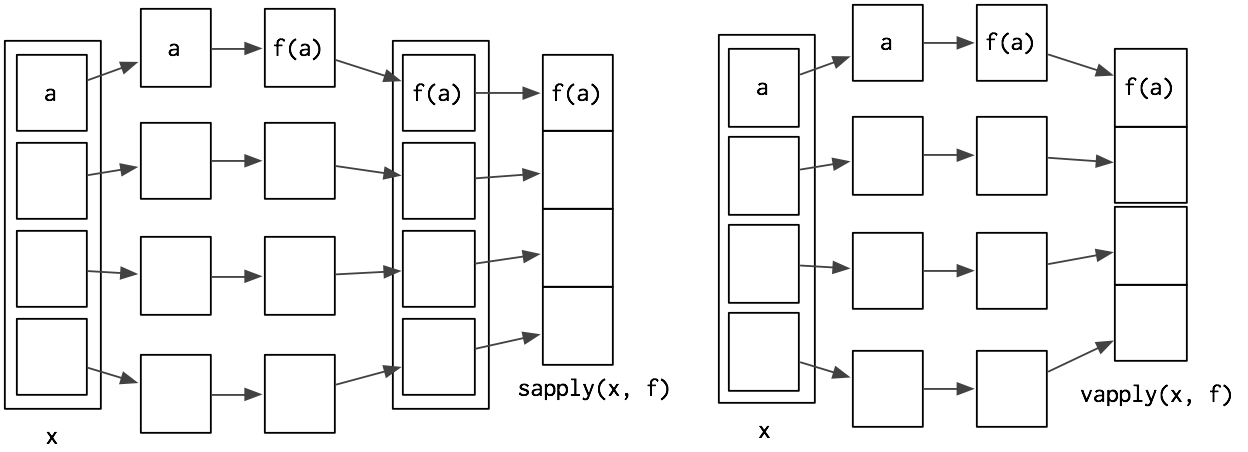
\includegraphics[width=5.67in]{diagrams/sapply-vapply.png}

\texttt{vapply()} and \texttt{sapply()} have different outputs from
\texttt{lapply()}. The following section discusses \texttt{Map()}, which
has different inputs.

\hypertarget{map}{%
\subsection{\texorpdfstring{Multiple inputs: \texttt{Map} (and
\texttt{mapply})}{Multiple inputs: Map (and mapply)}}\label{map}}

With \texttt{lapply()}, only one argument to the function varies; the
others are fixed. This makes it poorly suited for some problems. For
example, how would you find a weighted mean when you have two lists, one
of observations and the other of weights? \indexc{Map()}

\begin{Shaded}
\begin{Highlighting}[]
\CommentTok{# Generate some sample data}
\NormalTok{xs <-}\StringTok{ }\KeywordTok{replicate}\NormalTok{(}\DecValTok{5}\NormalTok{, }\KeywordTok{runif}\NormalTok{(}\DecValTok{10}\NormalTok{), }\DataTypeTok{simplify =} \OtherTok{FALSE}\NormalTok{)}
\NormalTok{ws <-}\StringTok{ }\KeywordTok{replicate}\NormalTok{(}\DecValTok{5}\NormalTok{, }\KeywordTok{rpois}\NormalTok{(}\DecValTok{10}\NormalTok{, }\DecValTok{5}\NormalTok{) }\OperatorTok{+}\StringTok{ }\DecValTok{1}\NormalTok{, }\DataTypeTok{simplify =} \OtherTok{FALSE}\NormalTok{)}
\end{Highlighting}
\end{Shaded}

It's easy to use \texttt{lapply()} to compute the unweighted means:

\begin{Shaded}
\begin{Highlighting}[]
\KeywordTok{unlist}\NormalTok{(}\KeywordTok{lapply}\NormalTok{(xs, mean))}
\end{Highlighting}
\end{Shaded}

\begin{verbatim}
## [1] 0.431 0.703 0.532 0.467 0.633
\end{verbatim}

But how could we supply the weights to \texttt{weighted.mean()}?
\texttt{lapply(x,\ means,\ w)} won't work because the additional
arguments to \texttt{lapply()} are passed to every call. We could change
looping forms:

\begin{Shaded}
\begin{Highlighting}[]
\KeywordTok{unlist}\NormalTok{(}\KeywordTok{lapply}\NormalTok{(}\KeywordTok{seq_along}\NormalTok{(xs), }\ControlFlowTok{function}\NormalTok{(i) \{}
  \KeywordTok{weighted.mean}\NormalTok{(xs[[i]], ws[[i]])}
\NormalTok{\}))}
\end{Highlighting}
\end{Shaded}

\begin{verbatim}
## [1] 0.463 0.695 0.542 0.446 0.627
\end{verbatim}

This works, but it's a little clumsy. A cleaner alternative is to use
\texttt{Map}, a variant of \texttt{lapply()}, where all arguments can
vary. This lets us write:

\begin{Shaded}
\begin{Highlighting}[]
\KeywordTok{unlist}\NormalTok{(}\KeywordTok{Map}\NormalTok{(weighted.mean, xs, ws))}
\end{Highlighting}
\end{Shaded}

\begin{verbatim}
## [1] 0.463 0.695 0.542 0.446 0.627
\end{verbatim}

Note that the order of arguments is a little different: function is the
first argument for \texttt{Map()} and the second for \texttt{lapply()}.

This is equivalent to:

\begin{Shaded}
\begin{Highlighting}[]
\KeywordTok{stopifnot}\NormalTok{(}\KeywordTok{length}\NormalTok{(xs) }\OperatorTok{==}\StringTok{ }\KeywordTok{length}\NormalTok{(ws))}
\NormalTok{out <-}\StringTok{ }\KeywordTok{vector}\NormalTok{(}\StringTok{"list"}\NormalTok{, }\KeywordTok{length}\NormalTok{(xs))}
\ControlFlowTok{for}\NormalTok{ (i }\ControlFlowTok{in} \KeywordTok{seq_along}\NormalTok{(xs)) \{}
\NormalTok{  out[[i]] <-}\StringTok{ }\KeywordTok{weighted.mean}\NormalTok{(xs[[i]], ws[[i]])}
\NormalTok{\}}
\end{Highlighting}
\end{Shaded}

There's a natural equivalence between \texttt{Map()} and
\texttt{lapply()} because you can always convert a \texttt{Map()} to an
\texttt{lapply()} that iterates over indices. But using \texttt{Map()}
is more concise, and more clearly indicates what you're trying to do.

\texttt{Map} is useful whenever you have two (or more) lists (or data
frames) that you need to process in parallel. For example, another way
of standardising columns is to first compute the means and then divide
by them. We could do this with \texttt{lapply()}, but if we do it in two
steps, we can more easily check the results at each step, which is
particularly important if the first step is more complicated.

\begin{Shaded}
\begin{Highlighting}[]
\NormalTok{mtmeans <-}\StringTok{ }\KeywordTok{lapply}\NormalTok{(mtcars, mean)}
\NormalTok{mtmeans[] <-}\StringTok{ }\KeywordTok{Map}\NormalTok{(}\StringTok{`}\DataTypeTok{/}\StringTok{`}\NormalTok{, mtcars, mtmeans)}

\CommentTok{# In this case, equivalent to}
\NormalTok{mtcars[] <-}\StringTok{ }\KeywordTok{lapply}\NormalTok{(mtcars, }\ControlFlowTok{function}\NormalTok{(x) x }\OperatorTok{/}\StringTok{ }\KeywordTok{mean}\NormalTok{(x))}
\end{Highlighting}
\end{Shaded}

If some of the arguments should be fixed and constant, use an anonymous
function:

\begin{Shaded}
\begin{Highlighting}[]
\KeywordTok{Map}\NormalTok{(}\ControlFlowTok{function}\NormalTok{(x, w) }\KeywordTok{weighted.mean}\NormalTok{(x, w, }\DataTypeTok{na.rm =} \OtherTok{TRUE}\NormalTok{), xs, ws)}
\end{Highlighting}
\end{Shaded}

We'll see a more compact way to express the same idea in the next
chapter.

\begin{shortbox}\Boxhead{mapply}

You may be more familiar with \texttt{mapply()} than \texttt{Map()}. I
prefer \texttt{Map()} because:

\begin{itemize}
\item
  It's equivalent to \texttt{mapply} with \texttt{simplify\ =\ FALSE},
  which is almost always what you want.
\item
  Instead of using an anonymous function to provide constant inputs,
  \texttt{mapply} has the \texttt{MoreArgs} argument that takes a list
  of extra arguments that will be supplied, as is, to each call. This
  breaks R's usual lazy evaluation semantics, and is inconsistent with
  other functions.
\end{itemize}

In brief, \texttt{mapply()} adds more complication for little gain.
\indexc{mapply()}

\end{shortbox}

\hypertarget{rolling-computations}{%
\subsection{Rolling computations}\label{rolling-computations}}

What if you need a for loop replacement that doesn't exist in base R?
You can often create your own by recognising common looping structures
and implementing your own wrapper. For example, you might be interested
in smoothing your data using a rolling (or running) mean function:
\index{rolling calculation}

\begin{Shaded}
\begin{Highlighting}[]
\NormalTok{rollmean <-}\StringTok{ }\ControlFlowTok{function}\NormalTok{(x, n) \{}
\NormalTok{  out <-}\StringTok{ }\KeywordTok{rep}\NormalTok{(}\OtherTok{NA}\NormalTok{, }\KeywordTok{length}\NormalTok{(x))}

\NormalTok{  offset <-}\StringTok{ }\KeywordTok{trunc}\NormalTok{(n }\OperatorTok{/}\StringTok{ }\DecValTok{2}\NormalTok{)}
  \ControlFlowTok{for}\NormalTok{ (i }\ControlFlowTok{in}\NormalTok{ (offset }\OperatorTok{+}\StringTok{ }\DecValTok{1}\NormalTok{)}\OperatorTok{:}\NormalTok{(}\KeywordTok{length}\NormalTok{(x) }\OperatorTok{-}\StringTok{ }\NormalTok{n }\OperatorTok{+}\StringTok{ }\NormalTok{offset }\OperatorTok{+}\StringTok{ }\DecValTok{1}\NormalTok{)) \{}
\NormalTok{    out[i] <-}\StringTok{ }\KeywordTok{mean}\NormalTok{(x[(i }\OperatorTok{-}\StringTok{ }\NormalTok{offset)}\OperatorTok{:}\NormalTok{(i }\OperatorTok{+}\StringTok{ }\NormalTok{offset }\OperatorTok{-}\StringTok{ }\DecValTok{1}\NormalTok{)])}
\NormalTok{  \}}
\NormalTok{  out}
\NormalTok{\}}
\NormalTok{x <-}\StringTok{ }\KeywordTok{seq}\NormalTok{(}\DecValTok{1}\NormalTok{, }\DecValTok{3}\NormalTok{, }\DataTypeTok{length =} \FloatTok{1e2}\NormalTok{) }\OperatorTok{+}\StringTok{ }\KeywordTok{runif}\NormalTok{(}\FloatTok{1e2}\NormalTok{)}
\KeywordTok{plot}\NormalTok{(x)}
\KeywordTok{lines}\NormalTok{(}\KeywordTok{rollmean}\NormalTok{(x, }\DecValTok{5}\NormalTok{), }\DataTypeTok{col =} \StringTok{"blue"}\NormalTok{, }\DataTypeTok{lwd =} \DecValTok{2}\NormalTok{)}
\KeywordTok{lines}\NormalTok{(}\KeywordTok{rollmean}\NormalTok{(x, }\DecValTok{10}\NormalTok{), }\DataTypeTok{col =} \StringTok{"red"}\NormalTok{, }\DataTypeTok{lwd =} \DecValTok{2}\NormalTok{)}
\end{Highlighting}
\end{Shaded}

\includegraphics{/home/elio/Documents/adv-r/book/tex/Functionals_files/figure-latex/roll-mean-1.png}

But if the noise was more variable (i.e., it has a longer tail), you
might worry that your rolling mean was too sensitive to outliers.
Instead, you might want to compute a rolling median.

\begin{Shaded}
\begin{Highlighting}[]
\NormalTok{x <-}\StringTok{ }\KeywordTok{seq}\NormalTok{(}\DecValTok{1}\NormalTok{, }\DecValTok{3}\NormalTok{, }\DataTypeTok{length =} \FloatTok{1e2}\NormalTok{) }\OperatorTok{+}\StringTok{ }\KeywordTok{rt}\NormalTok{(}\FloatTok{1e2}\NormalTok{, }\DataTypeTok{df =} \DecValTok{2}\NormalTok{) }\OperatorTok{/}\StringTok{ }\DecValTok{3}
\KeywordTok{plot}\NormalTok{(x)}
\KeywordTok{lines}\NormalTok{(}\KeywordTok{rollmean}\NormalTok{(x, }\DecValTok{5}\NormalTok{), }\DataTypeTok{col =} \StringTok{"red"}\NormalTok{, }\DataTypeTok{lwd =} \DecValTok{2}\NormalTok{)}
\end{Highlighting}
\end{Shaded}

\includegraphics{/home/elio/Documents/adv-r/book/tex/Functionals_files/figure-latex/outliers-1.png}

To change \texttt{rollmean()} to \texttt{rollmedian()}, all you need to
do is replace \texttt{mean} with \texttt{median} inside the loop. But
instead of copying and pasting to create a new function, we could
extract the idea of computing a rolling summary into its own function:
\indexc{rollapply()}

\begin{Shaded}
\begin{Highlighting}[]
\NormalTok{rollapply <-}\StringTok{ }\ControlFlowTok{function}\NormalTok{(x, n, f, ...) \{}
\NormalTok{  out <-}\StringTok{ }\KeywordTok{rep}\NormalTok{(}\OtherTok{NA}\NormalTok{, }\KeywordTok{length}\NormalTok{(x))}

\NormalTok{  offset <-}\StringTok{ }\KeywordTok{trunc}\NormalTok{(n }\OperatorTok{/}\StringTok{ }\DecValTok{2}\NormalTok{)}
  \ControlFlowTok{for}\NormalTok{ (i }\ControlFlowTok{in}\NormalTok{ (offset }\OperatorTok{+}\StringTok{ }\DecValTok{1}\NormalTok{)}\OperatorTok{:}\NormalTok{(}\KeywordTok{length}\NormalTok{(x) }\OperatorTok{-}\StringTok{ }\NormalTok{n }\OperatorTok{+}\StringTok{ }\NormalTok{offset }\OperatorTok{+}\StringTok{ }\DecValTok{1}\NormalTok{)) \{}
\NormalTok{    out[i] <-}\StringTok{ }\KeywordTok{f}\NormalTok{(x[(i }\OperatorTok{-}\StringTok{ }\NormalTok{offset)}\OperatorTok{:}\NormalTok{(i }\OperatorTok{+}\StringTok{ }\NormalTok{offset }\OperatorTok{-}\StringTok{ }\DecValTok{1}\NormalTok{)], ...)}
\NormalTok{  \}}
\NormalTok{  out}
\NormalTok{\}}
\KeywordTok{plot}\NormalTok{(x)}
\KeywordTok{lines}\NormalTok{(}\KeywordTok{rollapply}\NormalTok{(x, }\DecValTok{5}\NormalTok{, median), }\DataTypeTok{col =} \StringTok{"red"}\NormalTok{, }\DataTypeTok{lwd =} \DecValTok{2}\NormalTok{)}
\end{Highlighting}
\end{Shaded}

\includegraphics{/home/elio/Documents/adv-r/book/tex/Functionals_files/figure-latex/roll-apply-1.png}

You might notice that the internal loop looks pretty similar to a
\texttt{vapply()} loop, so we could rewrite the function as:

\begin{Shaded}
\begin{Highlighting}[]
\NormalTok{rollapply <-}\StringTok{ }\ControlFlowTok{function}\NormalTok{(x, n, f, ...) \{}
\NormalTok{  offset <-}\StringTok{ }\KeywordTok{trunc}\NormalTok{(n }\OperatorTok{/}\StringTok{ }\DecValTok{2}\NormalTok{)}
\NormalTok{  locs <-}\StringTok{ }\NormalTok{(offset }\OperatorTok{+}\StringTok{ }\DecValTok{1}\NormalTok{)}\OperatorTok{:}\NormalTok{(}\KeywordTok{length}\NormalTok{(x) }\OperatorTok{-}\StringTok{ }\NormalTok{n }\OperatorTok{+}\StringTok{ }\NormalTok{offset }\OperatorTok{+}\StringTok{ }\DecValTok{1}\NormalTok{)}
\NormalTok{  num <-}\StringTok{ }\KeywordTok{vapply}\NormalTok{(}
\NormalTok{    locs, }
    \ControlFlowTok{function}\NormalTok{(i) }\KeywordTok{f}\NormalTok{(x[(i }\OperatorTok{-}\StringTok{ }\NormalTok{offset)}\OperatorTok{:}\NormalTok{(i }\OperatorTok{+}\StringTok{ }\NormalTok{offset)], ...),}
    \KeywordTok{numeric}\NormalTok{(}\DecValTok{1}\NormalTok{)}
\NormalTok{  )}

  \KeywordTok{c}\NormalTok{(}\KeywordTok{rep}\NormalTok{(}\OtherTok{NA}\NormalTok{, offset), num)}
\NormalTok{\}}
\end{Highlighting}
\end{Shaded}

This is effectively the same as the implementation in
\texttt{zoo::rollapply()}, which provides many more features and much
more error checking.

\hypertarget{parallelisation}{%
\subsection{Parallelisation}\label{parallelisation}}

One interesting thing about the implementation of \texttt{lapply()} is
that because each iteration is isolated from all others, the order in
which they are computed doesn't matter. For example, \texttt{lapply3()}
scrambles the order of computation, but the results are always the same:
\index{parallel computing} \index{multicore}

\begin{Shaded}
\begin{Highlighting}[]
\NormalTok{lapply3 <-}\StringTok{ }\ControlFlowTok{function}\NormalTok{(x, f, ...) \{}
\NormalTok{  out <-}\StringTok{ }\KeywordTok{vector}\NormalTok{(}\StringTok{"list"}\NormalTok{, }\KeywordTok{length}\NormalTok{(x))}
  \ControlFlowTok{for}\NormalTok{ (i }\ControlFlowTok{in} \KeywordTok{sample}\NormalTok{(}\KeywordTok{seq_along}\NormalTok{(x))) \{}
\NormalTok{    out[[i]] <-}\StringTok{ }\KeywordTok{f}\NormalTok{(x[[i]], ...)}
\NormalTok{  \}}
\NormalTok{  out}
\NormalTok{\}}
\KeywordTok{unlist}\NormalTok{(}\KeywordTok{lapply}\NormalTok{(}\DecValTok{1}\OperatorTok{:}\DecValTok{10}\NormalTok{, sqrt))}
\end{Highlighting}
\end{Shaded}

\begin{verbatim}
##  [1] 1.00 1.41 1.73 2.00 2.24 2.45 2.65 2.83 3.00 3.16
\end{verbatim}

\begin{Shaded}
\begin{Highlighting}[]
\KeywordTok{unlist}\NormalTok{(}\KeywordTok{lapply3}\NormalTok{(}\DecValTok{1}\OperatorTok{:}\DecValTok{10}\NormalTok{, sqrt))}
\end{Highlighting}
\end{Shaded}

\begin{verbatim}
##  [1] 1.00 1.41 1.73 2.00 2.24 2.45 2.65 2.83 3.00 3.16
\end{verbatim}

This has a very important consequence: since we can compute each element
in any order, it's easy to dispatch the tasks to different cores, and
compute them in parallel. This is what \texttt{parallel::mclapply()}
(and \texttt{parallel::mcMap()}) does. (These functions are not
available in Windows, but you can use the similar \texttt{parLapply()}
with a bit more work. See \protect\hyperlink{parallelise}{parallelise}
for more details.) \indexc{mclapply()}

\begin{Shaded}
\begin{Highlighting}[]
\KeywordTok{library}\NormalTok{(parallel)}
\KeywordTok{unlist}\NormalTok{(}\KeywordTok{mclapply}\NormalTok{(}\DecValTok{1}\OperatorTok{:}\DecValTok{10}\NormalTok{, sqrt, }\DataTypeTok{mc.cores =} \DecValTok{4}\NormalTok{))}
\end{Highlighting}
\end{Shaded}

\begin{verbatim}
##  [1] 1.00 1.41 1.73 2.00 2.24 2.45 2.65 2.83 3.00 3.16
\end{verbatim}

In this case, \texttt{mclapply()} is actually slower than
\texttt{lapply()}. This is because the cost of the individual
computations is low, and additional work is needed to send the
computation to the different cores and to collect the results.

If we take a more realistic example, generating bootstrap replicates of
a linear model for example, the advantages are clearer:
\index{bootstrapping}

\begin{Shaded}
\begin{Highlighting}[]
\NormalTok{boot_df <-}\StringTok{ }\ControlFlowTok{function}\NormalTok{(x) x[}\KeywordTok{sample}\NormalTok{(}\KeywordTok{nrow}\NormalTok{(x), }\DataTypeTok{rep =}\NormalTok{ T), ]}
\NormalTok{rsquared <-}\StringTok{ }\ControlFlowTok{function}\NormalTok{(mod) }\KeywordTok{summary}\NormalTok{(mod)}\OperatorTok{$}\NormalTok{r.square}
\NormalTok{boot_lm <-}\StringTok{ }\ControlFlowTok{function}\NormalTok{(i) \{}
  \KeywordTok{rsquared}\NormalTok{(}\KeywordTok{lm}\NormalTok{(mpg }\OperatorTok{~}\StringTok{ }\NormalTok{wt }\OperatorTok{+}\StringTok{ }\NormalTok{disp, }\DataTypeTok{data =} \KeywordTok{boot_df}\NormalTok{(mtcars)))}
\NormalTok{\}}

\KeywordTok{system.time}\NormalTok{(}\KeywordTok{lapply}\NormalTok{(}\DecValTok{1}\OperatorTok{:}\DecValTok{500}\NormalTok{, boot_lm))}
\end{Highlighting}
\end{Shaded}

\begin{verbatim}
##    user  system elapsed 
##   1.381   0.019   1.422
\end{verbatim}

\begin{Shaded}
\begin{Highlighting}[]
\KeywordTok{system.time}\NormalTok{(}\KeywordTok{mclapply}\NormalTok{(}\DecValTok{1}\OperatorTok{:}\DecValTok{500}\NormalTok{, boot_lm, }\DataTypeTok{mc.cores =} \DecValTok{2}\NormalTok{))}
\end{Highlighting}
\end{Shaded}

\begin{verbatim}
##    user  system elapsed 
##   0.000   0.007   0.783
\end{verbatim}

While increasing the number of cores will not always lead to linear
improvement, switching from \texttt{lapply()} or \texttt{Map()} to its
parallelised forms can dramatically improve computational performance.

\hypertarget{exercises-1}{%
\subsection{Exercises}\label{exercises-1}}

\begin{enumerate}
\def\labelenumi{\arabic{enumi}.}
\item
  Use \texttt{vapply()} to:

  \begin{enumerate}
  \def\labelenumii{\alph{enumii})}
  \item
    Compute the standard deviation of every column in a numeric data
    frame.
  \item
    Compute the standard deviation of every numeric column in a mixed
    data frame. (Hint: you'll need to use \texttt{vapply()} twice.)
  \end{enumerate}
\item
  Why is using \texttt{sapply()} to get the \texttt{class()} of each
  element in a data frame dangerous?
\item
  The following code simulates the performance of a t-test for
  non-normal data. Use \texttt{sapply()} and an anonymous function to
  extract the p-value from every trial.

\begin{Shaded}
\begin{Highlighting}[]
\NormalTok{trials <-}\StringTok{ }\KeywordTok{replicate}\NormalTok{(}
  \DecValTok{100}\NormalTok{, }
  \KeywordTok{t.test}\NormalTok{(}\KeywordTok{rpois}\NormalTok{(}\DecValTok{10}\NormalTok{, }\DecValTok{10}\NormalTok{), }\KeywordTok{rpois}\NormalTok{(}\DecValTok{7}\NormalTok{, }\DecValTok{10}\NormalTok{)),}
  \DataTypeTok{simplify =} \OtherTok{FALSE}
\NormalTok{)}
\end{Highlighting}
\end{Shaded}

  Extra challenge: get rid of the anonymous function by using
  \texttt{{[}{[}} directly.
\item
  What does \texttt{replicate()} do? What sort of for loop does it
  eliminate? Why do its arguments differ from \texttt{lapply()} and
  friends?
\item
  Implement a version of \texttt{lapply()} that supplies \texttt{FUN}
  with both the name and the value of each component.
\item
  Implement a combination of \texttt{Map()} and \texttt{vapply()} to
  create an \texttt{lapply()} variant that iterates in parallel over all
  of its inputs and stores its outputs in a vector (or a matrix). What
  arguments should the function take?
\item
  Implement \texttt{mcsapply()}, a multicore version of
  \texttt{sapply()}. Can you implement \texttt{mcvapply()}, a parallel
  version of \texttt{vapply()}? Why or why not?
\end{enumerate}

\hypertarget{functionals-ds}{%
\section{Manipulating matrices and data frames}\label{functionals-ds}}

Functionals can also be used to eliminate loops in common data
manipulation tasks. In this section, we'll give a brief overview of the
available options, hint at how they can help you, and point you in the
right direction to learn more. We'll cover three categories of data
structure functionals:

\begin{itemize}
\item
  \texttt{apply()}, \texttt{sweep()}, and \texttt{outer()} work with
  matrices.
\item
  \texttt{tapply()} summarises a vector by groups defined by another
  vector.
\item
  the \texttt{plyr} package, which generalises \texttt{tapply()} to make
  it easy to work with data frames, lists, or arrays as inputs, and data
  frames, lists, or arrays as outputs.
\end{itemize}

\hypertarget{matrix-and-array-operations}{%
\subsection{Matrix and array
operations}\label{matrix-and-array-operations}}

So far, all the functionals we've seen work with 1d input structures.
The three functionals in this section provide useful tools for working
with higher-dimensional data structures. \texttt{apply()} is a variant
of \texttt{sapply()} that works with matrices and arrays. You can think
of it as an operation that summarises a matrix or array by collapsing
each row or column to a single number. It has four arguments:
\indexc{apply()}

\begin{itemize}
\tightlist
\item
  \texttt{X}, the matrix or array to summarise
\item
  \texttt{MARGIN}, an integer vector giving the dimensions to summarise
  over, 1 = rows, 2 = columns, etc.
\item
  \texttt{FUN}, a summary function
\item
  \texttt{...} other arguments passed on to \texttt{FUN}
\end{itemize}

A typical example of \texttt{apply()} looks like this

\begin{Shaded}
\begin{Highlighting}[]
\NormalTok{a <-}\StringTok{ }\KeywordTok{matrix}\NormalTok{(}\DecValTok{1}\OperatorTok{:}\DecValTok{20}\NormalTok{, }\DataTypeTok{nrow =} \DecValTok{5}\NormalTok{)}
\KeywordTok{apply}\NormalTok{(a, }\DecValTok{1}\NormalTok{, mean)}
\end{Highlighting}
\end{Shaded}

\begin{verbatim}
## [1]  8.5  9.5 10.5 11.5 12.5
\end{verbatim}

\begin{Shaded}
\begin{Highlighting}[]
\KeywordTok{apply}\NormalTok{(a, }\DecValTok{2}\NormalTok{, mean)}
\end{Highlighting}
\end{Shaded}

\begin{verbatim}
## [1]  3  8 13 18
\end{verbatim}

There are a few caveats to using \texttt{apply()}. It doesn't have a
simplify argument, so you can never be completely sure what type of
output you'll get. This means that \texttt{apply()} is not safe to use
inside a function unless you carefully check the inputs.
\texttt{apply()} is also not idempotent in the sense that if the summary
function is the identity operator, the output is not always the same as
the input:

\begin{Shaded}
\begin{Highlighting}[]
\NormalTok{a1 <-}\StringTok{ }\KeywordTok{apply}\NormalTok{(a, }\DecValTok{1}\NormalTok{, identity)}
\KeywordTok{identical}\NormalTok{(a, a1)}
\end{Highlighting}
\end{Shaded}

\begin{verbatim}
## [1] FALSE
\end{verbatim}

\begin{Shaded}
\begin{Highlighting}[]
\KeywordTok{identical}\NormalTok{(a, }\KeywordTok{t}\NormalTok{(a1))}
\end{Highlighting}
\end{Shaded}

\begin{verbatim}
## [1] TRUE
\end{verbatim}

\begin{Shaded}
\begin{Highlighting}[]
\NormalTok{a2 <-}\StringTok{ }\KeywordTok{apply}\NormalTok{(a, }\DecValTok{2}\NormalTok{, identity)}
\KeywordTok{identical}\NormalTok{(a, a2)}
\end{Highlighting}
\end{Shaded}

\begin{verbatim}
## [1] TRUE
\end{verbatim}

(You can put high-dimensional arrays back in the right order using
\texttt{aperm()}, or use \texttt{plyr::aaply()}, which is idempotent.)

\texttt{sweep()} allows you to ``sweep'' out the values of a summary
statistic. It is often used with \texttt{apply()} to standardise arrays.
The following example scales the rows of a matrix so that all values lie
between 0 and 1. \indexc{sweep()}

\begin{Shaded}
\begin{Highlighting}[]
\NormalTok{x <-}\StringTok{ }\KeywordTok{matrix}\NormalTok{(}\KeywordTok{rnorm}\NormalTok{(}\DecValTok{20}\NormalTok{, }\DecValTok{0}\NormalTok{, }\DecValTok{10}\NormalTok{), }\DataTypeTok{nrow =} \DecValTok{4}\NormalTok{)}
\NormalTok{x1 <-}\StringTok{ }\KeywordTok{sweep}\NormalTok{(x, }\DecValTok{1}\NormalTok{, }\KeywordTok{apply}\NormalTok{(x, }\DecValTok{1}\NormalTok{, min), }\StringTok{`}\DataTypeTok{-}\StringTok{`}\NormalTok{)}
\NormalTok{x2 <-}\StringTok{ }\KeywordTok{sweep}\NormalTok{(x1, }\DecValTok{1}\NormalTok{, }\KeywordTok{apply}\NormalTok{(x1, }\DecValTok{1}\NormalTok{, max), }\StringTok{`}\DataTypeTok{/}\StringTok{`}\NormalTok{)}
\end{Highlighting}
\end{Shaded}

The final matrix functional is \texttt{outer()}. It's a little different
in that it takes multiple vector inputs and creates a matrix or array
output where the input function is run over every combination of the
inputs: \indexc{outer()}

\begin{Shaded}
\begin{Highlighting}[]
\CommentTok{# Create a times table}
\KeywordTok{outer}\NormalTok{(}\DecValTok{1}\OperatorTok{:}\DecValTok{3}\NormalTok{, }\DecValTok{1}\OperatorTok{:}\DecValTok{10}\NormalTok{, }\StringTok{"*"}\NormalTok{)}
\end{Highlighting}
\end{Shaded}

\begin{verbatim}
##      [,1] [,2] [,3] [,4] [,5] [,6] [,7] [,8] [,9] [,10]
## [1,]    1    2    3    4    5    6    7    8    9    10
## [2,]    2    4    6    8   10   12   14   16   18    20
## [3,]    3    6    9   12   15   18   21   24   27    30
\end{verbatim}

Good places to learn more about \texttt{apply()} and friends are:

\begin{itemize}
\item
  \href{http://petewerner.blogspot.com/2012/12/using-apply-sapply-lapply-in-r.html}{``Using
  apply, sapply, lapply in R''} by Peter Werner.
\item
  \href{http://rforpublichealth.blogspot.no/2012/09/the-infamous-apply-function.html}{``The
  infamous apply function''} by Slawa Rokicki.
\item
  \href{http://forgetfulfunctor.blogspot.com/2011/07/r-apply-function-tutorial-with-examples.html}{``The
  R apply function - a tutorial with examples''} by axiomOfChoice.
\item
  The stackoverflow question
  \href{http://stackoverflow.com/questions/3505701}{``R Grouping
  functions: \texttt{sapply} vs. \texttt{lapply} vs. \texttt{apply} vs.
  \texttt{tapply} vs. \texttt{by} vs. \texttt{aggregate}''}.
\end{itemize}

\hypertarget{group-apply}{%
\subsection{Group apply}\label{group-apply}}

You can think about \texttt{tapply()} as a generalisation to
\texttt{apply()} that allows for ``ragged'' arrays, arrays where each
row can have a different number of columns. This is often needed when
you're trying to summarise a data set. For example, imagine you've
collected pulse rate data from a medical trial, and you want to compare
the two groups: \indexc{tapply()}

\begin{Shaded}
\begin{Highlighting}[]
\NormalTok{pulse <-}\StringTok{ }\KeywordTok{round}\NormalTok{(}\KeywordTok{rnorm}\NormalTok{(}\DecValTok{22}\NormalTok{, }\DecValTok{70}\NormalTok{, }\DecValTok{10} \OperatorTok{/}\StringTok{ }\DecValTok{3}\NormalTok{)) }\OperatorTok{+}\StringTok{ }\KeywordTok{rep}\NormalTok{(}\KeywordTok{c}\NormalTok{(}\DecValTok{0}\NormalTok{, }\DecValTok{5}\NormalTok{), }\KeywordTok{c}\NormalTok{(}\DecValTok{10}\NormalTok{, }\DecValTok{12}\NormalTok{))}
\NormalTok{group <-}\StringTok{ }\KeywordTok{rep}\NormalTok{(}\KeywordTok{c}\NormalTok{(}\StringTok{"A"}\NormalTok{, }\StringTok{"B"}\NormalTok{), }\KeywordTok{c}\NormalTok{(}\DecValTok{10}\NormalTok{, }\DecValTok{12}\NormalTok{))}

\KeywordTok{tapply}\NormalTok{(pulse, group, length)}
\end{Highlighting}
\end{Shaded}

\begin{verbatim}
##  A  B 
## 10 12
\end{verbatim}

\begin{Shaded}
\begin{Highlighting}[]
\KeywordTok{tapply}\NormalTok{(pulse, group, mean)}
\end{Highlighting}
\end{Shaded}

\begin{verbatim}
##    A    B 
## 72.4 76.3
\end{verbatim}

\texttt{tapply()} works by creating a ``ragged'' data structure from a
set of inputs, and then applying a function to the individual elements
of that structure. The first task is actually what the \texttt{split()}
function does. It takes two inputs and returns a list which groups
elements together from the first vector according to elements, or
categories, from the second vector:

\begin{Shaded}
\begin{Highlighting}[]
\KeywordTok{split}\NormalTok{(pulse, group)}
\end{Highlighting}
\end{Shaded}

\begin{verbatim}
## $A
##  [1] 74 75 70 74 70 71 75 73 71 71
## 
## $B
##  [1] 72 79 75 70 78 74 76 83 82 73 76 78
\end{verbatim}

Then \texttt{tapply()} is just the combination of \texttt{split()} and
\texttt{sapply()}:

\begin{Shaded}
\begin{Highlighting}[]
\NormalTok{tapply2 <-}\StringTok{ }\ControlFlowTok{function}\NormalTok{(x, group, f, ..., }\DataTypeTok{simplify =} \OtherTok{TRUE}\NormalTok{) \{}
\NormalTok{  pieces <-}\StringTok{ }\KeywordTok{split}\NormalTok{(x, group)}
  \KeywordTok{sapply}\NormalTok{(pieces, f, }\DataTypeTok{simplify =}\NormalTok{ simplify)}
\NormalTok{\}}
\KeywordTok{tapply2}\NormalTok{(pulse, group, length)}
\end{Highlighting}
\end{Shaded}

\begin{verbatim}
##  A  B 
## 10 12
\end{verbatim}

\begin{Shaded}
\begin{Highlighting}[]
\KeywordTok{tapply2}\NormalTok{(pulse, group, mean)}
\end{Highlighting}
\end{Shaded}

\begin{verbatim}
##    A    B 
## 72.4 76.3
\end{verbatim}

Being able to rewrite \texttt{tapply()} as a combination of
\texttt{split()} and \texttt{sapply()} is a good indication that we've
identified some useful building blocks. \indexc{split()}

\hypertarget{the-plyr-package}{%
\subsection{The plyr package}\label{the-plyr-package}}

One challenge with using the base functionals is that they have grown
organically over time, and have been written by multiple authors. This
means that they are not very consistent: \index{plyr}

\begin{itemize}
\item
  With \texttt{tapply()} and \texttt{sapply()}, the simplify argument is
  called \texttt{simplify}. With \texttt{mapply()}, it's called
  \texttt{SIMPLIFY}. With \texttt{apply()}, the argument is absent.
\item
  \texttt{vapply()} is a variant of \texttt{sapply()} that allows you to
  describe what the output should be, but there are no corresponding
  variants for \texttt{tapply()}, \texttt{apply()}, or \texttt{Map()}.
\item
  The first argument of most base functionals is a vector, but the first
  argument in \texttt{Map()} is a function.
\end{itemize}

This makes learning these operators challenging, as you have to memorise
all of the variations. Additionally, if you think about the possible
combinations of input and output types, base R only covers a partial set
of cases:

\begin{longtable}[]{@{}llll@{}}
\toprule
& list & data frame & array\tabularnewline
\midrule
\endhead
list & \texttt{lapply()} & & \texttt{sapply()}\tabularnewline
data frame & \texttt{by()} & &\tabularnewline
array & & & \texttt{apply()}\tabularnewline
\bottomrule
\end{longtable}

This was one of the driving motivations behind the creation of the plyr
package. It provides consistently named functions with consistently
named arguments and covers all combinations of input and output data
structures:

\begin{longtable}[]{@{}llll@{}}
\toprule
& list & data frame & array\tabularnewline
\midrule
\endhead
list & \texttt{llply()} & \texttt{ldply()} &
\texttt{laply()}\tabularnewline
data frame & \texttt{dlply()} & \texttt{ddply()} &
\texttt{daply()}\tabularnewline
array & \texttt{alply()} & \texttt{adply()} &
\texttt{aaply()}\tabularnewline
\bottomrule
\end{longtable}

Each of these functions splits up the input, applies a function to each
piece, and then combines the results. Overall, this process is called
``split-apply-combine''. You can read more about it and plyr in
\href{http://www.jstatsoft.org/v40/i01/}{``The Split-Apply-Combine
Strategy for Data Analysis''}, an open-access article published in the
\emph{Journal of Statistical Software}.
\index{split-apply-combine strategy}

\hypertarget{exercises-2}{%
\subsection{Exercises}\label{exercises-2}}

\begin{enumerate}
\def\labelenumi{\arabic{enumi}.}
\item
  How does \texttt{apply()} arrange the output? Read the documentation
  and perform some experiments.
\item
  There's no equivalent to \texttt{split()} + \texttt{vapply()}. Should
  there be? When would it be useful? Implement one yourself.
\item
  Implement a pure R version of \texttt{split()}. (Hint: use
  \texttt{unique()} and subsetting.) Can you do it without a for loop?
\item
  What other types of input and output are missing? Brainstorm before
  you look up some answers in the
  \href{http://www.jstatsoft.org/v40/i01/}{plyr paper}.
\end{enumerate}

\hypertarget{functionals-fp}{%
\section{Manipulating lists}\label{functionals-fp}}

Another way of thinking about functionals is as a set of general tools
for altering, subsetting, and collapsing lists. Every functional
programming language has three tools for this: \texttt{Map()},
\texttt{Reduce()}, and \texttt{Filter()}. We've seen \texttt{Map()}
already, and the following sections describe \texttt{Reduce()}, a
powerful tool for extending two-argument functions, and
\texttt{Filter()}, a member of an important class of functionals that
work with predicates, functions that return a single \texttt{TRUE} or
\texttt{FALSE}.

\hypertarget{reduce}{%
\subsection{\texorpdfstring{\texttt{Reduce()}}{Reduce()}}\label{reduce}}

\texttt{Reduce()} reduces a vector, \texttt{x}, to a single value by
recursively calling a function, \texttt{f}, two arguments at a time. It
combines the first two elements with \texttt{f}, then combines the
result of that call with the third element, and so on. Calling
\texttt{Reduce(f,\ 1:3)} is equivalent to \texttt{f(f(1,\ 2),\ 3)}.
Reduce is also known as fold, because it folds together adjacent
elements in the list. \indexc{Reduce()} \index{fold}

The following two examples show what \texttt{Reduce} does with an infix
and prefix function:

\begin{Shaded}
\begin{Highlighting}[]
\KeywordTok{Reduce}\NormalTok{(}\StringTok{`}\DataTypeTok{+}\StringTok{`}\NormalTok{, }\DecValTok{1}\OperatorTok{:}\DecValTok{3}\NormalTok{) }\CommentTok{# -> ((1 + 2) + 3)}
\KeywordTok{Reduce}\NormalTok{(sum, }\DecValTok{1}\OperatorTok{:}\DecValTok{3}\NormalTok{) }\CommentTok{# -> sum(sum(1, 2), 3)}
\end{Highlighting}
\end{Shaded}

The essence of \texttt{Reduce()} can be described by a simple for loop:

\begin{Shaded}
\begin{Highlighting}[]
\NormalTok{Reduce2 <-}\StringTok{ }\ControlFlowTok{function}\NormalTok{(f, x) \{}
\NormalTok{  out <-}\StringTok{ }\NormalTok{x[[}\DecValTok{1}\NormalTok{]]}
  \ControlFlowTok{for}\NormalTok{(i }\ControlFlowTok{in} \KeywordTok{seq}\NormalTok{(}\DecValTok{2}\NormalTok{, }\KeywordTok{length}\NormalTok{(x))) \{}
\NormalTok{    out <-}\StringTok{ }\KeywordTok{f}\NormalTok{(out, x[[i]])}
\NormalTok{  \}}
\NormalTok{  out}
\NormalTok{\}}
\end{Highlighting}
\end{Shaded}

The real \texttt{Reduce()} is more complicated because it includes
arguments to control whether the values are reduced from the left or
from the right (\texttt{right}), an optional initial value
(\texttt{init}), and an option to output intermediate results
(\texttt{accumulate}).

\texttt{Reduce()} is an elegant way of extending a function that works
with two inputs into a function that can deal with any number of inputs.
It's useful for implementing many types of recursive operations, like
merges and intersections. (We'll see another use in the final case
study.) Imagine you have a list of numeric vectors, and you want to find
the values that occur in every element:

\begin{Shaded}
\begin{Highlighting}[]
\NormalTok{l <-}\StringTok{ }\KeywordTok{replicate}\NormalTok{(}\DecValTok{5}\NormalTok{, }\KeywordTok{sample}\NormalTok{(}\DecValTok{1}\OperatorTok{:}\DecValTok{10}\NormalTok{, }\DecValTok{15}\NormalTok{, }\DataTypeTok{replace =}\NormalTok{ T), }\DataTypeTok{simplify =} \OtherTok{FALSE}\NormalTok{)}
\KeywordTok{str}\NormalTok{(l)}
\end{Highlighting}
\end{Shaded}

\begin{verbatim}
## List of 5
##  $ : int [1:15] 3 6 7 1 6 1 8 2 5 9 ...
##  $ : int [1:15] 9 6 2 8 4 2 4 1 1 10 ...
##  $ : int [1:15] 8 2 5 1 10 10 10 9 3 1 ...
##  $ : int [1:15] 5 9 7 9 1 1 2 10 6 3 ...
##  $ : int [1:15] 2 2 4 1 3 4 4 9 9 7 ...
\end{verbatim}

You could do that by intersecting each element in turn:

\begin{Shaded}
\begin{Highlighting}[]
\KeywordTok{intersect}\NormalTok{(}\KeywordTok{intersect}\NormalTok{(}\KeywordTok{intersect}\NormalTok{(}\KeywordTok{intersect}\NormalTok{(l[[}\DecValTok{1}\NormalTok{]], l[[}\DecValTok{2}\NormalTok{]]),}
\NormalTok{  l[[}\DecValTok{3}\NormalTok{]]), l[[}\DecValTok{4}\NormalTok{]]), l[[}\DecValTok{5}\NormalTok{]])}
\end{Highlighting}
\end{Shaded}

\begin{verbatim}
## [1] 3 1 2 9
\end{verbatim}

That's hard to read. With \texttt{Reduce()}, the equivalent is:

\begin{Shaded}
\begin{Highlighting}[]
\KeywordTok{Reduce}\NormalTok{(intersect, l)}
\end{Highlighting}
\end{Shaded}

\begin{verbatim}
## [1] 3 1 2 9
\end{verbatim}

\hypertarget{predicate-functionals}{%
\subsection{Predicate functionals}\label{predicate-functionals}}

A \textbf{predicate} is a function that returns a single \texttt{TRUE}
or \texttt{FALSE}, like \texttt{is.character}, \texttt{all}, or
\texttt{is.NULL}. A predicate functional applies a predicate to each
element of a list or data frame. There are three useful predicate
functionals in base R: \texttt{Filter()}, \texttt{Find()}, and
\texttt{Position()}. \index{predicates}
\index{functions!predict|see{predicates}}

\begin{itemize}
\item
  \texttt{Filter()} selects only those elements which match the
  predicate. \indexc{Filter()}
\item
  \texttt{Find()} returns the first element which matches the predicate
  (or the last element if \texttt{right\ =\ TRUE}). \indexc{Find()}
\item
  \texttt{Position()} returns the position of the first element that
  matches the predicate (or the last element if
  \texttt{right\ =\ TRUE}). \indexc{Position()}
\end{itemize}

Another useful predicate functional is \texttt{where()}, a custom
functional that generates a logical vector from a list (or a data frame)
and a predicate: \indexc{where()}

\begin{Shaded}
\begin{Highlighting}[]
\NormalTok{where <-}\StringTok{ }\ControlFlowTok{function}\NormalTok{(f, x) \{}
  \KeywordTok{vapply}\NormalTok{(x, f, }\KeywordTok{logical}\NormalTok{(}\DecValTok{1}\NormalTok{))}
\NormalTok{\}}
\end{Highlighting}
\end{Shaded}

The following example shows how you might use these functionals with a
data frame:

\begin{Shaded}
\begin{Highlighting}[]
\NormalTok{df <-}\StringTok{ }\KeywordTok{data.frame}\NormalTok{(}\DataTypeTok{x =} \DecValTok{1}\OperatorTok{:}\DecValTok{3}\NormalTok{, }\DataTypeTok{y =} \KeywordTok{c}\NormalTok{(}\StringTok{"a"}\NormalTok{, }\StringTok{"b"}\NormalTok{, }\StringTok{"c"}\NormalTok{))}
\KeywordTok{where}\NormalTok{(is.factor, df)}
\end{Highlighting}
\end{Shaded}

\begin{verbatim}
##     x     y 
## FALSE  TRUE
\end{verbatim}

\begin{Shaded}
\begin{Highlighting}[]
\KeywordTok{str}\NormalTok{(}\KeywordTok{Filter}\NormalTok{(is.factor, df))}
\end{Highlighting}
\end{Shaded}

\begin{verbatim}
## 'data.frame':    3 obs. of  1 variable:
##  $ y: Factor w/ 3 levels "a","b","c": 1 2 3
\end{verbatim}

\begin{Shaded}
\begin{Highlighting}[]
\KeywordTok{str}\NormalTok{(}\KeywordTok{Find}\NormalTok{(is.factor, df))}
\end{Highlighting}
\end{Shaded}

\begin{verbatim}
##  Factor w/ 3 levels "a","b","c": 1 2 3
\end{verbatim}

\begin{Shaded}
\begin{Highlighting}[]
\KeywordTok{Position}\NormalTok{(is.factor, df)}
\end{Highlighting}
\end{Shaded}

\begin{verbatim}
## [1] 2
\end{verbatim}

\hypertarget{exercises-3}{%
\subsection{Exercises}\label{exercises-3}}

\begin{enumerate}
\def\labelenumi{\arabic{enumi}.}
\item
  Why isn't \texttt{is.na()} a predicate function? What base R function
  is closest to being a predicate version of \texttt{is.na()}?
\item
  Use \texttt{Filter()} and \texttt{vapply()} to create a function that
  applies a summary statistic to every numeric column in a data frame.
\item
  What's the relationship between \texttt{which()} and
  \texttt{Position()}? What's the relationship between \texttt{where()}
  and \texttt{Filter()}?
\item
  Implement \texttt{Any()}, a function that takes a list and a predicate
  function, and returns \texttt{TRUE} if the predicate function returns
  \texttt{TRUE} for any of the inputs. Implement \texttt{All()}
  similarly.
\item
  Implement the \texttt{span()} function from Haskell: given a list
  \texttt{x} and a predicate function \texttt{f}, \texttt{span} returns
  the location of the longest sequential run of elements where the
  predicate is true. (Hint: you might find \texttt{rle()} helpful.)
\end{enumerate}

\hypertarget{functionals-math}{%
\section{Mathematical functionals}\label{functionals-math}}

Functionals are very common in mathematics. The limit, the maximum, the
roots (the set of points where \texttt{f(x)\ =\ 0}), and the definite
integral are all functionals: given a function, they return a single
number (or vector of numbers). At first glance, these functions don't
seem to fit in with the theme of eliminating loops, but if you dig
deeper you'll find out that they are all implemented using an algorithm
that involves iteration.

In this section we'll use some of R's built-in mathematical functionals.
There are three functionals that work with functions to return single
numeric values: \indexc{integrate()} \indexc{uniroot()}
\indexc{optimise()}

\begin{itemize}
\tightlist
\item
  \texttt{integrate()} finds the area under the curve defined by
  \texttt{f()}
\item
  \texttt{uniroot()} finds where \texttt{f()} hits zero
\item
  \texttt{optimise()} finds the location of lowest (or highest) value of
  \texttt{f()}
\end{itemize}

Let's explore how these are used with a simple function, \texttt{sin()}:

\begin{Shaded}
\begin{Highlighting}[]
\KeywordTok{integrate}\NormalTok{(sin, }\DecValTok{0}\NormalTok{, pi)}
\end{Highlighting}
\end{Shaded}

\begin{verbatim}
## 2 with absolute error < 2.2e-14
\end{verbatim}

\begin{Shaded}
\begin{Highlighting}[]
\KeywordTok{str}\NormalTok{(}\KeywordTok{uniroot}\NormalTok{(sin, pi }\OperatorTok{*}\StringTok{ }\KeywordTok{c}\NormalTok{(}\DecValTok{1} \OperatorTok{/}\StringTok{ }\DecValTok{2}\NormalTok{, }\DecValTok{3} \OperatorTok{/}\StringTok{ }\DecValTok{2}\NormalTok{)))}
\end{Highlighting}
\end{Shaded}

\begin{verbatim}
## List of 5
##  $ root      : num 3.14
##  $ f.root    : num 1.22e-16
##  $ iter      : int 2
##  $ init.it   : int NA
##  $ estim.prec: num 6.1e-05
\end{verbatim}

\begin{Shaded}
\begin{Highlighting}[]
\KeywordTok{str}\NormalTok{(}\KeywordTok{optimise}\NormalTok{(sin, }\KeywordTok{c}\NormalTok{(}\DecValTok{0}\NormalTok{, }\DecValTok{2} \OperatorTok{*}\StringTok{ }\NormalTok{pi)))}
\end{Highlighting}
\end{Shaded}

\begin{verbatim}
## List of 2
##  $ minimum  : num 4.71
##  $ objective: num -1
\end{verbatim}

\begin{Shaded}
\begin{Highlighting}[]
\KeywordTok{str}\NormalTok{(}\KeywordTok{optimise}\NormalTok{(sin, }\KeywordTok{c}\NormalTok{(}\DecValTok{0}\NormalTok{, pi), }\DataTypeTok{maximum =} \OtherTok{TRUE}\NormalTok{))}
\end{Highlighting}
\end{Shaded}

\begin{verbatim}
## List of 2
##  $ maximum  : num 1.57
##  $ objective: num 1
\end{verbatim}

In statistics, optimisation is often used for maximum likelihood
estimation (MLE). In MLE, we have two sets of parameters: the data,
which is fixed for a given problem, and the parameters, which vary as we
try to find the maximum. These two sets of parameters make the problem
well suited for closures. Combining closures with optimisation gives
rise to the following approach to solving MLE problems.
\index{maximum likelihood}

The following example shows how we might find the maximum likelihood
estimate for \(\lambda\), if our data come from a Poisson distribution.
First, we create a function factory that, given a dataset, returns a
function that computes the negative log likelihood (NLL) for parameter
\texttt{lambda}. In R, it's common to work with the negative since
\texttt{optimise()} defaults to finding the minimum.
\index{closures!maximum likelihood}

\begin{Shaded}
\begin{Highlighting}[]
\NormalTok{poisson_nll <-}\StringTok{ }\ControlFlowTok{function}\NormalTok{(x) \{}
\NormalTok{  n <-}\StringTok{ }\KeywordTok{length}\NormalTok{(x)}
\NormalTok{  sum_x <-}\StringTok{ }\KeywordTok{sum}\NormalTok{(x)}
  \ControlFlowTok{function}\NormalTok{(lambda) \{}
\NormalTok{    n }\OperatorTok{*}\StringTok{ }\NormalTok{lambda }\OperatorTok{-}\StringTok{ }\NormalTok{sum_x }\OperatorTok{*}\StringTok{ }\KeywordTok{log}\NormalTok{(lambda) }\CommentTok{# + terms not involving lambda}
\NormalTok{  \}}
\NormalTok{\}}
\end{Highlighting}
\end{Shaded}

Note how the closure allows us to precompute values that are constant
with respect to the data.

We can use this function factory to generate specific NLL functions for
input data. Then \texttt{optimise()} allows us to find the best values
(the maximum likelihood estimates), given a generous starting range.

\begin{Shaded}
\begin{Highlighting}[]
\NormalTok{x1 <-}\StringTok{ }\KeywordTok{c}\NormalTok{(}\DecValTok{41}\NormalTok{, }\DecValTok{30}\NormalTok{, }\DecValTok{31}\NormalTok{, }\DecValTok{38}\NormalTok{, }\DecValTok{29}\NormalTok{, }\DecValTok{24}\NormalTok{, }\DecValTok{30}\NormalTok{, }\DecValTok{29}\NormalTok{, }\DecValTok{31}\NormalTok{, }\DecValTok{38}\NormalTok{)}
\NormalTok{x2 <-}\StringTok{ }\KeywordTok{c}\NormalTok{(}\DecValTok{6}\NormalTok{, }\DecValTok{4}\NormalTok{, }\DecValTok{7}\NormalTok{, }\DecValTok{3}\NormalTok{, }\DecValTok{3}\NormalTok{, }\DecValTok{7}\NormalTok{, }\DecValTok{5}\NormalTok{, }\DecValTok{2}\NormalTok{, }\DecValTok{2}\NormalTok{, }\DecValTok{7}\NormalTok{, }\DecValTok{5}\NormalTok{, }\DecValTok{4}\NormalTok{, }\DecValTok{12}\NormalTok{, }\DecValTok{6}\NormalTok{, }\DecValTok{9}\NormalTok{)}
\NormalTok{nll1 <-}\StringTok{ }\KeywordTok{poisson_nll}\NormalTok{(x1)}
\NormalTok{nll2 <-}\StringTok{ }\KeywordTok{poisson_nll}\NormalTok{(x2)}

\KeywordTok{optimise}\NormalTok{(nll1, }\KeywordTok{c}\NormalTok{(}\DecValTok{0}\NormalTok{, }\DecValTok{100}\NormalTok{))}\OperatorTok{$}\NormalTok{minimum}
\end{Highlighting}
\end{Shaded}

\begin{verbatim}
## [1] 32.1
\end{verbatim}

\begin{Shaded}
\begin{Highlighting}[]
\KeywordTok{optimise}\NormalTok{(nll2, }\KeywordTok{c}\NormalTok{(}\DecValTok{0}\NormalTok{, }\DecValTok{100}\NormalTok{))}\OperatorTok{$}\NormalTok{minimum}
\end{Highlighting}
\end{Shaded}

\begin{verbatim}
## [1] 5.47
\end{verbatim}

We can check that these values are correct by comparing them to the
analytic solution: in this case, it's just the mean of the data, 32.1
and 5.467.

Another important mathematical functional is \texttt{optim()}. It is a
generalisation of \texttt{optimise()} that works with more than one
dimension. If you're interested in how it works, you might want to
explore the \texttt{Rvmmin} package, which provides a pure-R
implementation of \texttt{optim()}. Interestingly \texttt{Rvmmin} is no
slower than \texttt{optim()}, even though it is written in R, not C. For
this problem, the bottleneck lies not in controlling the optimisation
but with having to evaluate the function multiple times.
\indexc{optim()}

\hypertarget{exercises-4}{%
\subsection{Exercises}\label{exercises-4}}

\begin{enumerate}
\def\labelenumi{\arabic{enumi}.}
\item
  Implement \texttt{arg\_max()}. It should take a function and a vector
  of inputs, and return the elements of the input where the function
  returns the highest value. For example,
  \texttt{arg\_max(-10:5,\ function(x)\ x\ \^{}\ 2)} should return -10.
  \texttt{arg\_max(-5:5,\ function(x)\ x\ \^{}\ 2)} should return
  \texttt{c(-5,\ 5)}. Also implement the matching \texttt{arg\_min()}
  function.
\item
  Challenge: read about the
  \href{http://mitpress.mit.edu/sicp/full-text/book/book-Z-H-12.html\#\%_sec_1.3}{fixed
  point algorithm}. Complete the exercises using R.
\end{enumerate}

\hypertarget{functionals-not}{%
\section{Loops that should be left as is}\label{functionals-not}}

Some loops have no natural functional equivalent. In this section you'll
learn about three common cases: \index{loops!when to use}

\begin{itemize}
\tightlist
\item
  modifying in place
\item
  recursive functions
\item
  while loops
\end{itemize}

It's possible to torture these problems to use a functional, but it's
not a good idea. You'll create code that is harder to understand,
eliminating the main reason for using functionals in the first case.

\hypertarget{modifying-in-place}{%
\subsection{Modifying in place}\label{modifying-in-place}}

If you need to modify part of an existing data frame, it's often better
to use a for loop. For example, the following code performs a
variable-by-variable transformation by matching the names of a list of
functions to the names of variables in a data frame.

\begin{Shaded}
\begin{Highlighting}[]
\NormalTok{trans <-}\StringTok{ }\KeywordTok{list}\NormalTok{(}
  \DataTypeTok{disp =} \ControlFlowTok{function}\NormalTok{(x) x }\OperatorTok{*}\StringTok{ }\FloatTok{0.0163871}\NormalTok{,}
  \DataTypeTok{am =} \ControlFlowTok{function}\NormalTok{(x) }\KeywordTok{factor}\NormalTok{(x, }\DataTypeTok{labels =} \KeywordTok{c}\NormalTok{(}\StringTok{"auto"}\NormalTok{, }\StringTok{"manual"}\NormalTok{))}
\NormalTok{)}
\ControlFlowTok{for}\NormalTok{(var }\ControlFlowTok{in} \KeywordTok{names}\NormalTok{(trans)) \{}
\NormalTok{  mtcars[[var]] <-}\StringTok{ }\NormalTok{trans[[var]](mtcars[[var]])}
\NormalTok{\}}
\end{Highlighting}
\end{Shaded}

We wouldn't normally use \texttt{lapply()} to replace this loop
directly, but it is \emph{possible}. Just replace the loop with
\texttt{lapply()} by using \texttt{\textless{}\textless{}-}:
\indexc{<<-}

\begin{Shaded}
\begin{Highlighting}[]
\KeywordTok{lapply}\NormalTok{(}\KeywordTok{names}\NormalTok{(trans), }\ControlFlowTok{function}\NormalTok{(var) \{}
\NormalTok{  mtcars[[var]] <<-}\StringTok{ }\NormalTok{trans[[var]](mtcars[[var]])}
\NormalTok{\})}
\end{Highlighting}
\end{Shaded}

The for loop is gone, but the code is longer and much harder to
understand. The reader needs to understand
\texttt{\textless{}\textless{}-} and how
\texttt{x{[}{[}y{]}{]}\ \textless{}\textless{}-\ z} works (it's not
simple!). In short, we've taken a simple, easily understood for loop,
and turned it into something few people will understand: not a good
idea!

\hypertarget{recursive-relationships}{%
\subsection{Recursive relationships}\label{recursive-relationships}}

It's hard to convert a for loop into a functional when the relationship
between elements is not independent, or is defined recursively. For
example, exponential smoothing works by taking a weighted average of the
current and previous data points. The \texttt{exps()} function below
implements exponential smoothing with a for loop.
\index{recurrence relations}

\begin{Shaded}
\begin{Highlighting}[]
\NormalTok{exps <-}\StringTok{ }\ControlFlowTok{function}\NormalTok{(x, alpha) \{}
\NormalTok{  s <-}\StringTok{ }\KeywordTok{numeric}\NormalTok{(}\KeywordTok{length}\NormalTok{(x) }\OperatorTok{+}\StringTok{ }\DecValTok{1}\NormalTok{)}
  \ControlFlowTok{for}\NormalTok{ (i }\ControlFlowTok{in} \KeywordTok{seq_along}\NormalTok{(s)) \{}
    \ControlFlowTok{if}\NormalTok{ (i }\OperatorTok{==}\StringTok{ }\DecValTok{1}\NormalTok{) \{}
\NormalTok{      s[i] <-}\StringTok{ }\NormalTok{x[i]}
\NormalTok{    \} }\ControlFlowTok{else}\NormalTok{ \{}
\NormalTok{      s[i] <-}\StringTok{ }\NormalTok{alpha }\OperatorTok{*}\StringTok{ }\NormalTok{x[i] }\OperatorTok{+}\StringTok{ }\NormalTok{(}\DecValTok{1} \OperatorTok{-}\StringTok{ }\NormalTok{alpha) }\OperatorTok{*}\StringTok{ }\NormalTok{s[i }\OperatorTok{-}\StringTok{ }\DecValTok{1}\NormalTok{]}
\NormalTok{    \}}
\NormalTok{  \}}
\NormalTok{  s}
\NormalTok{\}}
\NormalTok{x <-}\StringTok{ }\KeywordTok{runif}\NormalTok{(}\DecValTok{6}\NormalTok{)}
\KeywordTok{exps}\NormalTok{(x, }\FloatTok{0.5}\NormalTok{)}
\end{Highlighting}
\end{Shaded}

\begin{verbatim}
## [1] 0.573 0.506 0.410 0.450 0.705 0.384    NA
\end{verbatim}

We can't eliminate the for loop because none of the functionals we've
seen allow the output at position \texttt{i} to depend on both the input
and output at position \texttt{i\ -\ 1}.

One way to eliminate the for loop in this case is to
\href{http://en.wikipedia.org/wiki/Recurrence_relation\#Solving}{solve
the recurrence relation} by removing the recursion and replacing it with
explicit references. This requires a new set of mathematical tools, and
is challenging, but it can pay off by producing a simpler function.

\hypertarget{while-loops}{%
\subsection{While loops}\label{while-loops}}

Another type of looping construct in R is the \texttt{while} loop. It
keeps running until some condition is met. \texttt{while} loops are more
general than \texttt{for} loops: you can rewrite every for loop as a
while loop, but you can't do the reverse. For example, we could turn
this for loop: \index{loops!while} \indexc{while}

\begin{Shaded}
\begin{Highlighting}[]
\ControlFlowTok{for}\NormalTok{ (i }\ControlFlowTok{in} \DecValTok{1}\OperatorTok{:}\DecValTok{10}\NormalTok{) }\KeywordTok{print}\NormalTok{(i)}
\end{Highlighting}
\end{Shaded}

into this while loop:

\begin{Shaded}
\begin{Highlighting}[]
\NormalTok{i <-}\StringTok{ }\DecValTok{1}
\ControlFlowTok{while}\NormalTok{(i }\OperatorTok{<=}\StringTok{ }\DecValTok{10}\NormalTok{) \{}
  \KeywordTok{print}\NormalTok{(i)}
\NormalTok{  i <-}\StringTok{ }\NormalTok{i }\OperatorTok{+}\StringTok{ }\DecValTok{1}
\NormalTok{\}}
\end{Highlighting}
\end{Shaded}

Not every while loop can be turned into a for loop because many while
loops don't know in advance how many times they will be run:

\begin{Shaded}
\begin{Highlighting}[]
\NormalTok{i <-}\StringTok{ }\DecValTok{0}
\ControlFlowTok{while}\NormalTok{(}\OtherTok{TRUE}\NormalTok{) \{}
  \ControlFlowTok{if}\NormalTok{ (}\KeywordTok{runif}\NormalTok{(}\DecValTok{1}\NormalTok{) }\OperatorTok{>}\StringTok{ }\FloatTok{0.9}\NormalTok{) }\ControlFlowTok{break}
\NormalTok{  i <-}\StringTok{ }\NormalTok{i }\OperatorTok{+}\StringTok{ }\DecValTok{1}
\NormalTok{\}}
\end{Highlighting}
\end{Shaded}

This is a common problem when you're writing simulations.

In this case we can remove the loop by recognising a special feature of
the problem. Here we're counting the number of successes before
Bernoulli trial with p = 0.1 fails. This is a geometric random variable,
so you could replace the code with
\texttt{i\ \textless{}-\ rgeom(1,\ 0.1)}. Reformulating the problem in
this way is hard to do in general, but you'll benefit greatly if you can
do it for your problem.

\hypertarget{function-family}{%
\section{A family of functions}\label{function-family}}

To finish off the chapter, this case study shows how you can use
functionals to take a simple building block and make it powerful and
general. I'll start with a simple idea, adding two numbers together, and
use functionals to extend it to summing multiple numbers, computing
parallel and cumulative sums, and summing across array dimensions.

We'll start by defining a very simple addition function, one which takes
two scalar arguments:

\begin{Shaded}
\begin{Highlighting}[]
\NormalTok{add <-}\StringTok{ }\ControlFlowTok{function}\NormalTok{(x, y) \{}
  \KeywordTok{stopifnot}\NormalTok{(}\KeywordTok{length}\NormalTok{(x) }\OperatorTok{==}\StringTok{ }\DecValTok{1}\NormalTok{, }\KeywordTok{length}\NormalTok{(y) }\OperatorTok{==}\StringTok{ }\DecValTok{1}\NormalTok{,}
    \KeywordTok{is.numeric}\NormalTok{(x), }\KeywordTok{is.numeric}\NormalTok{(y))}
\NormalTok{  x }\OperatorTok{+}\StringTok{ }\NormalTok{y}
\NormalTok{\}}
\end{Highlighting}
\end{Shaded}

(We're using R's existing addition operator here, which does much more,
but the focus here is on how we can take very simple building blocks and
extend them to do more.)

I'll also add an \texttt{na.rm} argument. A helper function will make
this a bit easier: if \texttt{x} is missing it should return \texttt{y},
if \texttt{y} is missing it should return \texttt{x}, and if both
\texttt{x} and \texttt{y} are missing then it should return another
argument to the function: \texttt{identity}. This function is probably a
bit more general than what we need now, but it's useful if we implement
other binary operators.

\begin{Shaded}
\begin{Highlighting}[]
\NormalTok{rm_na <-}\StringTok{ }\ControlFlowTok{function}\NormalTok{(x, y, identity) \{}
  \ControlFlowTok{if}\NormalTok{ (}\KeywordTok{is.na}\NormalTok{(x) }\OperatorTok{&&}\StringTok{ }\KeywordTok{is.na}\NormalTok{(y)) \{}
\NormalTok{    identity}
\NormalTok{  \} }\ControlFlowTok{else} \ControlFlowTok{if}\NormalTok{ (}\KeywordTok{is.na}\NormalTok{(x)) \{}
\NormalTok{    y}
\NormalTok{  \} }\ControlFlowTok{else}\NormalTok{ \{}
\NormalTok{    x}
\NormalTok{  \}}
\NormalTok{\}}
\KeywordTok{rm_na}\NormalTok{(}\OtherTok{NA}\NormalTok{, }\DecValTok{10}\NormalTok{, }\DecValTok{0}\NormalTok{)}
\end{Highlighting}
\end{Shaded}

\begin{verbatim}
## [1] 10
\end{verbatim}

\begin{Shaded}
\begin{Highlighting}[]
\KeywordTok{rm_na}\NormalTok{(}\DecValTok{10}\NormalTok{, }\OtherTok{NA}\NormalTok{, }\DecValTok{0}\NormalTok{)}
\end{Highlighting}
\end{Shaded}

\begin{verbatim}
## [1] 10
\end{verbatim}

\begin{Shaded}
\begin{Highlighting}[]
\KeywordTok{rm_na}\NormalTok{(}\OtherTok{NA}\NormalTok{, }\OtherTok{NA}\NormalTok{, }\DecValTok{0}\NormalTok{)}
\end{Highlighting}
\end{Shaded}

\begin{verbatim}
## [1] 0
\end{verbatim}

This allows us to write a version of \texttt{add()} that can deal with
missing values if needed:

\begin{Shaded}
\begin{Highlighting}[]
\NormalTok{add <-}\StringTok{ }\ControlFlowTok{function}\NormalTok{(x, y, }\DataTypeTok{na.rm =} \OtherTok{FALSE}\NormalTok{) \{}
  \ControlFlowTok{if}\NormalTok{ (na.rm }\OperatorTok{&&}\StringTok{ }\NormalTok{(}\KeywordTok{is.na}\NormalTok{(x) }\OperatorTok{||}\StringTok{ }\KeywordTok{is.na}\NormalTok{(y))) }\KeywordTok{rm_na}\NormalTok{(x, y, }\DecValTok{0}\NormalTok{) }\ControlFlowTok{else}\NormalTok{ x }\OperatorTok{+}\StringTok{ }\NormalTok{y}
\NormalTok{\}}
\KeywordTok{add}\NormalTok{(}\DecValTok{10}\NormalTok{, }\OtherTok{NA}\NormalTok{)}
\end{Highlighting}
\end{Shaded}

\begin{verbatim}
## [1] NA
\end{verbatim}

\begin{Shaded}
\begin{Highlighting}[]
\KeywordTok{add}\NormalTok{(}\DecValTok{10}\NormalTok{, }\OtherTok{NA}\NormalTok{, }\DataTypeTok{na.rm =} \OtherTok{TRUE}\NormalTok{)}
\end{Highlighting}
\end{Shaded}

\begin{verbatim}
## [1] 10
\end{verbatim}

\begin{Shaded}
\begin{Highlighting}[]
\KeywordTok{add}\NormalTok{(}\OtherTok{NA}\NormalTok{, }\OtherTok{NA}\NormalTok{)}
\end{Highlighting}
\end{Shaded}

\begin{verbatim}
## [1] NA
\end{verbatim}

\begin{Shaded}
\begin{Highlighting}[]
\KeywordTok{add}\NormalTok{(}\OtherTok{NA}\NormalTok{, }\OtherTok{NA}\NormalTok{, }\DataTypeTok{na.rm =} \OtherTok{TRUE}\NormalTok{)}
\end{Highlighting}
\end{Shaded}

\begin{verbatim}
## [1] 0
\end{verbatim}

Why did we pick an identity of \texttt{0}? Why should
\texttt{add(NA,\ NA,\ na.rm\ =\ TRUE)} return 0? Well, for every other
input it returns a number, so even if both arguments are \texttt{NA}, it
should still do that. What number should it return? We can figure it out
because addition is associative, which means that the order of addition
doesn't matter. That means that the following two function calls should
return the same value:

\begin{Shaded}
\begin{Highlighting}[]
\KeywordTok{add}\NormalTok{(}\KeywordTok{add}\NormalTok{(}\DecValTok{3}\NormalTok{, }\OtherTok{NA}\NormalTok{, }\DataTypeTok{na.rm =} \OtherTok{TRUE}\NormalTok{), }\OtherTok{NA}\NormalTok{, }\DataTypeTok{na.rm =} \OtherTok{TRUE}\NormalTok{)}
\end{Highlighting}
\end{Shaded}

\begin{verbatim}
## [1] 3
\end{verbatim}

\begin{Shaded}
\begin{Highlighting}[]
\KeywordTok{add}\NormalTok{(}\DecValTok{3}\NormalTok{, }\KeywordTok{add}\NormalTok{(}\OtherTok{NA}\NormalTok{, }\OtherTok{NA}\NormalTok{, }\DataTypeTok{na.rm =} \OtherTok{TRUE}\NormalTok{), }\DataTypeTok{na.rm =} \OtherTok{TRUE}\NormalTok{)}
\end{Highlighting}
\end{Shaded}

\begin{verbatim}
## [1] 3
\end{verbatim}

This implies that \texttt{add(NA,\ NA,\ na.rm\ =\ TRUE)} must be 0, and
hence \texttt{identity\ =\ 0} is the correct default.

Now that we have the basics working, we can extend the function to deal
with more complicated inputs. One obvious generalisation is to add more
than two numbers. We can do this by iteratively adding two numbers: if
the input is \texttt{c(1,\ 2,\ 3)} we compute
\texttt{add(add(1,\ 2),\ 3)}. This is a simple application of
\texttt{Reduce()}:

\begin{Shaded}
\begin{Highlighting}[]
\NormalTok{r_add <-}\StringTok{ }\ControlFlowTok{function}\NormalTok{(xs, }\DataTypeTok{na.rm =} \OtherTok{TRUE}\NormalTok{) \{}
  \KeywordTok{Reduce}\NormalTok{(}\ControlFlowTok{function}\NormalTok{(x, y) }\KeywordTok{add}\NormalTok{(x, y, }\DataTypeTok{na.rm =}\NormalTok{ na.rm), xs)}
\NormalTok{\}}
\KeywordTok{r_add}\NormalTok{(}\KeywordTok{c}\NormalTok{(}\DecValTok{1}\NormalTok{, }\DecValTok{4}\NormalTok{, }\DecValTok{10}\NormalTok{))}
\end{Highlighting}
\end{Shaded}

\begin{verbatim}
## [1] 15
\end{verbatim}

This looks good, but we need to test a few special cases:

\begin{Shaded}
\begin{Highlighting}[]
\KeywordTok{r_add}\NormalTok{(}\OtherTok{NA}\NormalTok{, }\DataTypeTok{na.rm =} \OtherTok{TRUE}\NormalTok{)}
\end{Highlighting}
\end{Shaded}

\begin{verbatim}
## [1] NA
\end{verbatim}

\begin{Shaded}
\begin{Highlighting}[]
\KeywordTok{r_add}\NormalTok{(}\KeywordTok{numeric}\NormalTok{())}
\end{Highlighting}
\end{Shaded}

\begin{verbatim}
## NULL
\end{verbatim}

These are incorrect. In the first case, we get a missing value even
though we've explicitly asked to ignore them. In the second case, we get
\texttt{NULL} instead of a length one numeric vector (as we do for every
other set of inputs).

The two problems are related. If we give \texttt{Reduce()} a length one
vector, it doesn't have anything to reduce, so it just returns the
input. If we give it an input of length zero, it always returns
\texttt{NULL}. The easiest way to fix this problem is to use the
\texttt{init} argument of \texttt{Reduce()}. This is added to the start
of every input vector:

\begin{Shaded}
\begin{Highlighting}[]
\NormalTok{r_add <-}\StringTok{ }\ControlFlowTok{function}\NormalTok{(xs, }\DataTypeTok{na.rm =} \OtherTok{TRUE}\NormalTok{) \{}
  \KeywordTok{Reduce}\NormalTok{(}\ControlFlowTok{function}\NormalTok{(x, y) }\KeywordTok{add}\NormalTok{(x, y, }\DataTypeTok{na.rm =}\NormalTok{ na.rm), xs, }\DataTypeTok{init =} \DecValTok{0}\NormalTok{)}
\NormalTok{\}}
\KeywordTok{r_add}\NormalTok{(}\KeywordTok{c}\NormalTok{(}\DecValTok{1}\NormalTok{, }\DecValTok{4}\NormalTok{, }\DecValTok{10}\NormalTok{))}
\end{Highlighting}
\end{Shaded}

\begin{verbatim}
## [1] 15
\end{verbatim}

\begin{Shaded}
\begin{Highlighting}[]
\KeywordTok{r_add}\NormalTok{(}\OtherTok{NA}\NormalTok{, }\DataTypeTok{na.rm =} \OtherTok{TRUE}\NormalTok{)}
\end{Highlighting}
\end{Shaded}

\begin{verbatim}
## [1] 0
\end{verbatim}

\begin{Shaded}
\begin{Highlighting}[]
\KeywordTok{r_add}\NormalTok{(}\KeywordTok{numeric}\NormalTok{())}
\end{Highlighting}
\end{Shaded}

\begin{verbatim}
## [1] 0
\end{verbatim}

\texttt{r\_add()} is equivalent to \texttt{sum()}.

It would be nice to have a vectorised version of \texttt{add()} so that
we can perform the addition of two vectors of numbers in element-wise
fashion. We could use \texttt{Map()} or \texttt{vapply()} to implement
this, but neither is perfect. \texttt{Map()} returns a list, instead of
a numeric vector, so we need to use \texttt{simplify2array()}.
\texttt{vapply()} returns a vector but it requires us to loop over a set
of indices.

\begin{Shaded}
\begin{Highlighting}[]
\NormalTok{v_add1 <-}\StringTok{ }\ControlFlowTok{function}\NormalTok{(x, y, }\DataTypeTok{na.rm =} \OtherTok{FALSE}\NormalTok{) \{}
  \KeywordTok{stopifnot}\NormalTok{(}\KeywordTok{length}\NormalTok{(x) }\OperatorTok{==}\StringTok{ }\KeywordTok{length}\NormalTok{(y), }\KeywordTok{is.numeric}\NormalTok{(x), }\KeywordTok{is.numeric}\NormalTok{(y))}
  \ControlFlowTok{if}\NormalTok{ (}\KeywordTok{length}\NormalTok{(x) }\OperatorTok{==}\StringTok{ }\DecValTok{0}\NormalTok{) }\KeywordTok{return}\NormalTok{(}\KeywordTok{numeric}\NormalTok{())}
  \KeywordTok{simplify2array}\NormalTok{(}
    \KeywordTok{Map}\NormalTok{(}\ControlFlowTok{function}\NormalTok{(x, y) }\KeywordTok{add}\NormalTok{(x, y, }\DataTypeTok{na.rm =}\NormalTok{ na.rm), x, y)}
\NormalTok{  )}
\NormalTok{\}}

\NormalTok{v_add2 <-}\StringTok{ }\ControlFlowTok{function}\NormalTok{(x, y, }\DataTypeTok{na.rm =} \OtherTok{FALSE}\NormalTok{) \{}
  \KeywordTok{stopifnot}\NormalTok{(}\KeywordTok{length}\NormalTok{(x) }\OperatorTok{==}\StringTok{ }\KeywordTok{length}\NormalTok{(y), }\KeywordTok{is.numeric}\NormalTok{(x), }\KeywordTok{is.numeric}\NormalTok{(y))}
  \KeywordTok{vapply}\NormalTok{(}\KeywordTok{seq_along}\NormalTok{(x), }\ControlFlowTok{function}\NormalTok{(i) }\KeywordTok{add}\NormalTok{(x[i], y[i], }\DataTypeTok{na.rm =}\NormalTok{ na.rm),}
    \KeywordTok{numeric}\NormalTok{(}\DecValTok{1}\NormalTok{))}
\NormalTok{\}}
\end{Highlighting}
\end{Shaded}

A few test cases help to ensure that it behaves as we expect. We're a
bit stricter than base R here because we don't do recycling. (You could
add that if you wanted, but I find that recycling is a frequent source
of silent bugs.)

\begin{Shaded}
\begin{Highlighting}[]
\CommentTok{# Both versions give the same results}
\KeywordTok{v_add1}\NormalTok{(}\DecValTok{1}\OperatorTok{:}\DecValTok{10}\NormalTok{, }\DecValTok{1}\OperatorTok{:}\DecValTok{10}\NormalTok{)}
\end{Highlighting}
\end{Shaded}

\begin{verbatim}
##  [1]  2  4  6  8 10 12 14 16 18 20
\end{verbatim}

\begin{Shaded}
\begin{Highlighting}[]
\KeywordTok{v_add1}\NormalTok{(}\KeywordTok{numeric}\NormalTok{(), }\KeywordTok{numeric}\NormalTok{())}
\end{Highlighting}
\end{Shaded}

\begin{verbatim}
## numeric(0)
\end{verbatim}

\begin{Shaded}
\begin{Highlighting}[]
\KeywordTok{v_add1}\NormalTok{(}\KeywordTok{c}\NormalTok{(}\DecValTok{1}\NormalTok{, }\OtherTok{NA}\NormalTok{), }\KeywordTok{c}\NormalTok{(}\DecValTok{1}\NormalTok{, }\OtherTok{NA}\NormalTok{))}
\end{Highlighting}
\end{Shaded}

\begin{verbatim}
## [1]  2 NA
\end{verbatim}

\begin{Shaded}
\begin{Highlighting}[]
\KeywordTok{v_add1}\NormalTok{(}\KeywordTok{c}\NormalTok{(}\DecValTok{1}\NormalTok{, }\OtherTok{NA}\NormalTok{), }\KeywordTok{c}\NormalTok{(}\DecValTok{1}\NormalTok{, }\OtherTok{NA}\NormalTok{), }\DataTypeTok{na.rm =} \OtherTok{TRUE}\NormalTok{)}
\end{Highlighting}
\end{Shaded}

\begin{verbatim}
## [1] 2 0
\end{verbatim}

Another variant of \texttt{add()} is the cumulative sum. We can
implement it with \texttt{Reduce()} by setting the \texttt{accumulate}
argument to \texttt{TRUE}:

\begin{Shaded}
\begin{Highlighting}[]
\NormalTok{c_add <-}\StringTok{ }\ControlFlowTok{function}\NormalTok{(xs, }\DataTypeTok{na.rm =} \OtherTok{FALSE}\NormalTok{) \{}
  \KeywordTok{Reduce}\NormalTok{(}\ControlFlowTok{function}\NormalTok{(x, y) }\KeywordTok{add}\NormalTok{(x, y, }\DataTypeTok{na.rm =}\NormalTok{ na.rm), xs,}
    \DataTypeTok{accumulate =} \OtherTok{TRUE}\NormalTok{)}
\NormalTok{\}}
\KeywordTok{c_add}\NormalTok{(}\DecValTok{1}\OperatorTok{:}\DecValTok{10}\NormalTok{)}
\end{Highlighting}
\end{Shaded}

\begin{verbatim}
##  [1]  1  3  6 10 15 21 28 36 45 55
\end{verbatim}

\begin{Shaded}
\begin{Highlighting}[]
\KeywordTok{c_add}\NormalTok{(}\DecValTok{10}\OperatorTok{:}\DecValTok{1}\NormalTok{)}
\end{Highlighting}
\end{Shaded}

\begin{verbatim}
##  [1] 10 19 27 34 40 45 49 52 54 55
\end{verbatim}

This is equivalent to \texttt{cumsum()}.

Finally, we might want to define addition for more complicated data
structures like matrices. We could create \texttt{row} and \texttt{col}
variants that sum across rows and columns, respectively, or we could go
the whole hog and define an array version that could sum across any
arbitrary set of dimensions. These are easily implemented as
combinations of \texttt{r\_add()} and \texttt{apply()}.

\begin{Shaded}
\begin{Highlighting}[]
\NormalTok{row_sum <-}\StringTok{ }\ControlFlowTok{function}\NormalTok{(x, }\DataTypeTok{na.rm =} \OtherTok{FALSE}\NormalTok{) \{}
  \KeywordTok{apply}\NormalTok{(x, }\DecValTok{1}\NormalTok{, r_add, }\DataTypeTok{na.rm =}\NormalTok{ na.rm)}
\NormalTok{\}}
\NormalTok{col_sum <-}\StringTok{ }\ControlFlowTok{function}\NormalTok{(x, }\DataTypeTok{na.rm =} \OtherTok{FALSE}\NormalTok{) \{}
  \KeywordTok{apply}\NormalTok{(x, }\DecValTok{2}\NormalTok{, r_add, }\DataTypeTok{na.rm =}\NormalTok{ na.rm)}
\NormalTok{\}}
\NormalTok{arr_sum <-}\StringTok{ }\ControlFlowTok{function}\NormalTok{(x, dim, }\DataTypeTok{na.rm =} \OtherTok{FALSE}\NormalTok{) \{}
  \KeywordTok{apply}\NormalTok{(x, dim, r_add, }\DataTypeTok{na.rm =}\NormalTok{ na.rm)}
\NormalTok{\}}
\end{Highlighting}
\end{Shaded}

The first two are equivalent to \texttt{rowSums()} and
\texttt{colSums()}.

If every function we have created has an existing equivalent in base R,
why did we bother? There are two main reasons:

\begin{itemize}
\item
  Since all variants were implemented by combining a simple binary
  operator (\texttt{add()}) and a well-tested functional
  (\texttt{Reduce()}, \texttt{Map()}, \texttt{apply()}), we know that
  our variants will behave consistently.
\item
  We can apply the same infrastructure to other operators, especially
  those that might not have the full suite of variants in base R.
\end{itemize}

The downside of this approach is that these implementations are not that
efficient. (For example, \texttt{colSums(x)} is much faster than
\texttt{apply(x,\ 2,\ sum)}.) However, even if they aren't that fast,
simple implementations are still a good starting point because they're
less likely to have bugs. When you create faster versions, you can
compare the results to make sure your fast versions are still correct.

If you enjoyed this section, you might also enjoy
\href{http://stevelosh.com/blog/2013/03/list-out-of-lambda/}{``List out
of lambda''}, a blog article by Steve Losh that shows how you can
produce high level language structures (like lists) out of more
primitive language features (like closures, aka lambdas).

\hypertarget{exercises-5}{%
\subsection{Exercises}\label{exercises-5}}

\begin{enumerate}
\def\labelenumi{\arabic{enumi}.}
\item
  Implement \texttt{smaller} and \texttt{larger} functions that, given
  two inputs, return either the smaller or the larger value. Implement
  \texttt{na.rm\ =\ TRUE}: what should the identity be? (Hint:
  \texttt{smaller(x,\ smaller(NA,\ NA,\ na.rm\ =\ TRUE),\ na.rm\ =\ TRUE)}
  must be \texttt{x}, so \texttt{smaller(NA,\ NA,\ na.rm\ =\ TRUE)} must
  be bigger than any other value of x.) Use \texttt{smaller} and
  \texttt{larger} to implement equivalents of \texttt{min()},
  \texttt{max()}, \texttt{pmin()}, \texttt{pmax()}, and new functions
  \texttt{row\_min()} and \texttt{row\_max()}.
\item
  Create a table that has \emph{and}, \emph{or}, \emph{add},
  \emph{multiply}, \emph{smaller}, and \emph{larger} in the columns and
  \emph{binary operator}, \emph{reducing variant}, \emph{vectorised
  variant}, and \emph{array variants} in the rows.

  \begin{enumerate}
  \def\labelenumii{\alph{enumii})}
  \item
    Fill in the cells with the names of base R functions that perform
    each of the roles.
  \item
    Compare the names and arguments of the existing R functions. How
    consistent are they? How could you improve them?
  \item
    Complete the matrix by implementing any missing functions.
  \end{enumerate}
\item
  How does \texttt{paste()} fit into this structure? What is the scalar
  binary function that underlies \texttt{paste()}? What are the
  \texttt{sep} and \texttt{collapse} arguments to \texttt{paste()}
  equivalent to? Are there any \texttt{paste} variants that don't have
  existing R implementations?
\end{enumerate}
